% FOUR-RQ REVISION; ORGANIZATION REFERENCE: DOI 10.1145/3695988
% Uses Neural_Code_Security_Survey_FINAL.bib. Review layout; publication metadata unassigned.

\documentclass[acmsmall,screen,review,nonacm]{acmart}

\AtBeginDocument{%
  \providecommand\BibTeX{{%
    Bib\TeX}}}

% Working draft: publication metadata will be supplied by ACM.
\setcopyright{none}
\acmJournal{CSUR}
\usepackage{amssymb}
\usepackage{xcolor}
\usepackage{tikz}
\usetikzlibrary{positioning,arrows.meta}
\usepackage{adjustbox}
\usepackage{array}
\usepackage{booktabs}
\usepackage{longtable}
\usepackage{placeins}
\usepackage{float}
\usepackage{needspace}
\usepackage{ragged2e}
\usepackage{tabularx}
\usepackage{amsmath}
\microtypesetup{expansion=false}
\setlength{\headheight}{20pt}

\newcolumntype{L}[1]{>{\RaggedRight\arraybackslash}p{#1}}
\newcolumntype{C}[1]{>{\Centering\arraybackslash}p{#1}}
\newcolumntype{Y}{>{\RaggedRight\arraybackslash}X}
\setlength{\emergencystretch}{2em}

% Author-requested working annotations. Card text is editable in author-notes.py.
% Set \showauthornotesfalse to hide the cards for a clean reading copy.
\newif\ifshowauthornotes
\showauthornotestrue
\newcommand{\authortodo}[1]{%
  \ifshowauthornotes
    \par\addvspace{4pt}\noindent
    \includegraphics[page=#1,width=\linewidth]{\authornotesfile}%
    \par\addvspace{4pt}
  \fi}
\IfFileExists{author-notes.pdf}
  {\def\authornotesfile{author-notes.pdf}}
  {\def\authornotesfile{manuscript/author-notes.pdf}}

\begin{document}

\title{Security and Robustness of Neural Code Systems: A Survey of Attack Surfaces, Defenses, and Evaluation}

\author{Bin Duan}
\email{b.duan@uq.edu.au}
\affiliation{
\institution{The University of Queensland} \city{Brisbane} \state{Queensland} \country{Australia}
}
\author{Guowei Yang}
\email{guowei.yang@uq.edu.au}
\affiliation{
\institution{The University of Queensland} \city{Brisbane} \state{Queensland} \country{Australia}
}

\begin{abstract}
Neural code systems face attacks through program inputs, training data, and the external context consumed by coding agents. We review 148 works available by 30 June 2026, comprising 219 evaluated contributions across attacks, risk measurements, defenses, and evaluation resources. We organize attacks by their entry into training state, current inference input, or runtime context, and examine output, privacy, and ecosystem risks separately. Our analysis connects each reported result to its outcome oracle and, for program transformations, its preservation contract. Construction arguments, paired tests, and local symbolic checks support different retained properties. Execution may assess benign utility, a malicious payload, or an agent action, with different implications for security. Within-study comparisons show that protection depends on the attack family and can reduce functional utility. The synthesis identifies opportunities for executable preservation collections, shared agent traces, adaptive evaluation, and versioned benchmarks.

\end{abstract}

\begin{CCSXML}
<ccs2012>
 <concept>
  <concept_id>10002978.10003022</concept_id>
  <concept_desc>Security and privacy~Software and application security</concept_desc>
  <concept_significance>500</concept_significance>
 </concept>
 <concept>
  <concept_id>10011007.10011074.10011099</concept_id>
  <concept_desc>Software and its engineering~Software verification and validation</concept_desc>
  <concept_significance>300</concept_significance>
 </concept>
 <concept>
  <concept_id>10010147.10010257</concept_id>
  <concept_desc>Computing methodologies~Machine learning</concept_desc>
  <concept_significance>300</concept_significance>
 </concept>
</ccs2012>
\end{CCSXML}

\ccsdesc[500]{Security and privacy~Software and application security}
\ccsdesc[300]{Software and its engineering~Software verification and validation}
\ccsdesc[300]{Computing methodologies~Machine learning}

\keywords{Neural Code Models, Code LLMs, Coding Agents, Adversarial Attacks, Backdoor Attacks, Data Poisoning, Prompt Injection, Runtime Context, Robustness, Secure Code Generation}

\maketitle

\section{Introduction}
\label{sec:intro}
\label{sec:related}

Neural code systems are used to classify programs, retrieve code, generate implementations, and carry out development tasks through external tools. Security studies have expanded with these capabilities. Early work examined whether changes that retain a program's behavior could alter a code model's prediction~\cite{yefet2020adversarial,zhang2020generating}. Studies of code LLMs subsequently investigated insecure suggestions, reproduction of training material, and poisoned completions~\cite{pearce2022asleep,ziegler2021recitation,schuster2021autocomplete}. Coding agents add repositories, retrieval stores, tool descriptions, and execution environments to this setting, allowing attacker-controlled content to influence actions as well as generated text~\cite{liu2025yourai,xie2025redteaming}.

The experiments differ in both attacker control and measured outcome: a changed prediction, an insecure suggestion, and an executed command are different security events. Existing surveys organize this literature by problem class, system type, security property, or lifecycle stage (Table~\ref{tab:surveys}). We connect these perspectives through the state an adversary can modify and the property an evaluation measures.

{\scriptsize
\renewcommand{\arraystretch}{1.10}
\setlength{\tabcolsep}{2.5pt}
\begin{table*}[tp]
\centering
\caption{Related surveys by system coverage and organizing perspective. Checkmarks indicate substantive coverage; ``--'' marks system forms outside the primary scope.}
\label{tab:surveys}
\begin{tabular}{@{}L{2.00cm}C{2cm}C{1.05cm}C{1.15cm}L{7.00cm}@{}}
\toprule
\textbf{Survey} &
\textbf{Task-specific code model} &
\textbf{Code LLM} &
\textbf{Coding agent} &
\textbf{Organizing perspective} \\
\midrule

Qu et al.~\cite{qu2024robustnesssurvey} &
\(\checkmark\) &
-- &
-- &
Attacker knowledge, attack scenario, victim task, perturbation type, and evaluation metric. \\
\midrule

Y.~Yang et al.~\cite{yang2024survey} &
\(\checkmark\) &
\(\checkmark\) &
-- &
Security property, attack family, threat model, and countermeasure. \\
\midrule

Chen et al.~\cite{securitycode2024slr} &
\(\checkmark\) &
\(\checkmark\) &
-- &
Models, attacks, defenses, datasets, metrics, and artifacts. \\
\midrule

Z.~Yang et al.~\cite{robustness2024llms} &
-- &
\(\checkmark\) &
-- &
Non-functional properties, including robustness, security, privacy, explainability, efficiency, and usability. \\
\midrule

Negri-Ribalta et al.~\cite{negriribalta2024securegeneration} &
-- &
\(\checkmark\) &
-- &
Security risks introduced by AI-generated code and possible mitigations. \\
\midrule

Basic and Giaretta~\cite{basic2026codesecurity} &
-- &
\(\checkmark\) &
-- &
Insecure code generation, vulnerability detection and repair, prompting strategies, and data poisoning. \\
\midrule

Qu et al.~\cite{qu2025backdoorsurvey} &
-- &
\(\checkmark\) &
-- &
Training settings, trigger designs, backdoor attacks, and defenses. \\
\midrule

She et al.~\cite{she2026pitfalls} &
\(\checkmark\) &
\(\checkmark\) &
-- &
Pitfalls in data, system design, evaluation, and deployment. \\
\midrule

Maloyan and Namiot~\cite{maloyan2026promptinjection} &
-- &
-- &
\(\checkmark\) &
Prompt injection through skills, tools, and protocol ecosystems. \\
\midrule

This survey &
\(\checkmark\) &
\(\checkmark\) &
\(\checkmark\) &
Classification of attacks by entry through the training state, current inference input, or runtime context; separate treatment of studies that observe existing risks; reported outcome measures and program-preservation checks. \\

\bottomrule
\end{tabular}
\end{table*}
}

Our corpus contains 148 works available by 30 June 2026 and 219 evaluated contributions: 75 attacks, 30 risk studies, 110 defenses, and 4 evaluation resources. A work can contribute several roles, such as an attack and its evaluated mitigation. The survey contributes:
\begin{itemize}
\item A system model relating task-specific models, code LLMs, and coding agents to three attacker entry points: training state, current inference input, and runtime context (RQ1).
\item A comparison of attack mechanisms at these entry points and measurements of output, privacy, and ecosystem risks (RQ2).
\item An analysis of defenses by protection target, mechanism, utility cost, and evaluated outcome (RQ3).
\item A synthesis of preservation checks, outcome oracles, benchmarks, and the conditions for comparing results (RQ4).
\end{itemize}

Section~\ref{sec:method} describes the review approach. Sections~\ref{sec:rq1}--\ref{sec:rq4} answer the RQs, followed by threats to validity, research opportunities, and conclusions.

\section{Approach}
\label{sec:method}

The review combines database searches, supplementary source checks, and snowballing to answer four questions.

\subsection{RQs}
\label{sec:rqs}
\begin{description}
\item[RQ1: Systems and boundaries.] Which system forms are evaluated, and where can attacker-controlled material enter?
\item[RQ2: Attacks and risks.] What mechanisms induce failures, and what existing security risks are measured?
\item[RQ3: Defenses.] What protection mechanisms are evaluated, against which threats and at what utility cost?
\item[RQ4: Evaluation.] What preservation checks, outcome oracles, resources, and protocols support the reported results?
\end{description}

\subsection{Search Strategy}
The initial collection used DBLP, arXiv, and conference and journal indices. Its exports and candidate-level screening log were not retained. A supplementary search on 19 October 2026 used a public web index restricted to DBLP and arXiv, retaining the availability cutoff of 30 June 2026. The companion package contains its 16 exact queries, returned entries, screening decisions, and source follow-ups.

Searches combined system terms (\emph{code model}, \emph{code LLM}, \emph{neural code}, \emph{source code}, \emph{code generation}, and \emph{coding agent}) with adversarial robustness, poisoning, backdoors, prompt injection, privacy, and secure-generation terms. Supplementary queries added coding assistants, runtime enforcement, retrieval, tool and skill injection, provenance, unlearning, and package hallucination. Strings were adapted to each source's search syntax.

The supplementary index returned 107 distinct entries: 18 author, venue, disambiguation, or documentation pages; 21 studies already in the corpus; 17 newly included works; five secondary reviews; five post-cutoff works; 40 scope exclusions; and one code-related work with unresolved pre-cutoff availability. Eligibility and protocol coding followed primary sources linked from these returns.

\subsection{Study Selection}
\subsubsection{Eligibility Criteria}
Primary works were eligible when they evaluated a task-specific code model, code LLM, or coding agent on a code-related attack, empirical security risk, defense, or repository-level resource reporting functional and security outcomes. Eligible sources included archival publications, preprints, and first-party technical reports with inspectable methods and measured results. We excluded generic LLM or agent studies without separate code-related results, conventional security techniques without a neural component, unevaluated proposals, and superseded versions. Secondary surveys informed discovery and positioning.

\subsubsection{Screening and Version Selection}
The initial collection used title/abstract screening and full-text assessment. Supplementary screening and primary-source checks were model-assisted. The records distinguish initial coding from subsequent changes and retain unresolved eligibility decisions. Final verification excluded five works, comprising seven contributions, whose complete protocols or correspondence to a pre-cutoff version could not be verified; the exclusion ledger gives the reasons.

% 作者待办 01：按实际记录补充 AI 工具、版本、输入材料与筛选/编码职责。
\authortodo{1}

\paragraph{Deduplication and version handling.}
We matched titles, authors, DOIs, and arXiv identifiers, merging preprints and archival publications into one work. Evidence uses versions available by 30 June 2026. ACW uses its August 2025 arXiv version 4, SET-Backdoor its December 2025 preprint, and scanner-feedback repair its June 2025 version; later scientific additions are excluded.

\subsection{Snowballing Search}
Backward and forward snowballing supplemented the initial collection; separate hit counts were not retained. Logged reference and primary-source follow-ups added Quiring et al.'s authorship attack, FunPoison, and Signature~\cite{quiring2019authorship,xiao2026funpoison,le2025signature}. Their discovery and eligibility records are separate from the 107 index returns.

\subsection{Data Extraction and Analysis}
\label{sec:corpus}

The corpus contains 148 works and 219 evaluated contributions. Each contribution represents a work and study role; attacks are split further when a work evaluates different entry surfaces. Variants, victim configurations, and defense baselines within one work-role evaluation remain grouped. FDI, for example, contributes retrieval and continual-training attacks plus a grouped screening evaluation. Un-Repair's proposed evaluation and Tambon et al.'s general functional-bug taxonomy remain background references~\cite{unrepairing2024,tambon2025bugs}.

We assign four roles: \emph{attack} for an intervention intended to induce failure, including fixed malicious-request benchmarks; \emph{risk study} for measurements of insecure generation, training-data exposure, or ecosystem properties; \emph{defense} for evaluated prevention, detection, or mitigation; and \emph{evaluation resource} for repository- or project-level benchmarks reporting functionality and security. Diagnostic membership and extraction probes belong to the risk role because they measure existing training-data relationships. The resulting records comprise 75 attacks, 30 risk studies, 110 defenses, and 4 resources.

\label{sec:coding}
Each record contains the study role, system form, mechanism, task, representation, result type, outcome oracle, and applicable attacker access and preservation checks (Table~\ref{tab:rq-extraction}). Result codes are \textsf{PRED} for labels, rankings, similarity scores, or detector decisions; \textsf{GEN} for generated code or text; \textsf{MIX} for both; \textsf{AGT} for evaluated actions; and \textsf{OBS} for artifact measurements without a victim-model query. Result type describes the measured output: SecRepoBench evaluates agent-returned code (\textsf{GEN}), while RedCode also evaluates agent actions (\textsf{AGT}). Sections~\ref{sec:threat:semantics} and~\ref{sec:outcome-evidence} define preservation and outcome codes.

Model knowledge is \textsf{WB} (white-box), \textsf{GB} (gray-box), or \textsf{BB} (black-box). Write access is \textsf{TDW} for training data, \textsf{MW} for model weights, or \textsf{RCW} for runtime context. Current-request control is represented by the inference-input surface.

The first author coded the initial table in two passes. Model-assisted primary-source checks subsequently covered all 219 records from 148 works: 205 protocol checks and 14 targeted checks (Table~\ref{tab:audit-coverage}). The companion data retain source versions, locators, decisions, and an author-review sheet; human confirmation remains pending. Author manuscripts and official experiment artifacts supply evidence attributed to their named versions. Counts and table views are generated from the active records.

% 作者待办 02：核实已有人工编码描述，补充实际复核人员、范围、数量及分歧处理。
\authortodo{2}

\begin{table}[t]
\centering
\caption{Extracted information and the RQs it supports.}
\label{tab:rq-extraction}
\begin{tabularx}{\columnwidth}{@{}L{1.0cm}Y L{2.6cm}@{}}
\toprule
\textbf{RQ} & \textbf{Information used in the synthesis} & \textbf{Analysis} \\
\midrule
1 & System form, result type, writable state, and entry point & System and boundary map \\
2 & Attack or risk role, mechanism, task, representation, access, and budget & Mechanism comparison \\
3 & Defense role, protection target, control mechanism, and reported utility & Defense coverage \\
4 & Benchmarks, preservation contract and support, outcome oracle, execution purpose, and source version & Evaluation comparison \\
\bottomrule
\end{tabularx}
\end{table}

\section{RQ1: What Neural Code Systems and Security Boundaries Have Been Studied?}
\label{sec:rq1}
\label{sec:threat}

The reviewed systems range from program prediction to generation and iterative tool use. Each exposes different state and interfaces to an adversary.

\subsection{Which System Forms Are Evaluated?}
Task-specific models provide services such as classification, retrieval, and summarization. Code LLMs support code and text tasks through prompting. Coding agents add repository state, retrieval, tools, and an execution loop (Table~\ref{tab:system-forms}). These are evaluated configurations: the same model can serve a task-specific interface or operate within an agent. Generation introduces sampled executable outputs; agents additionally turn outputs into actions on external state.

\begin{table*}[t]
\centering
\caption{Neural code system forms and the security boundary introduced by each form.}
\label{tab:system-forms}
\begin{tabularx}{\textwidth}{@{}L{2.6cm}L{3.1cm}L{3.6cm}Y@{}}
\toprule
\textbf{System form} & \textbf{Typical interface} & \textbf{State beyond the current request} & \textbf{Security consequence} \\
\midrule
Task-specific code model & Label, ranking, similarity, or summary & Model parameters and training data & Robustness depends on the permitted code transformation, model access, and task metric. \\
\midrule
Code LLM & Completion, patch, explanation, or generated program & Model parameters, training data, and sometimes retrieved context & Security includes generated-code functionality, weakness detection, memorization, and sampling policy. \\
\midrule
Coding agent & Iterative observations, plans, tool calls, and actions & Repository state, retrieval stores, rules, skills, tool descriptions, credentials, and execution environment & Security depends on the full trust path from external context to authorization, execution, and terminal effect. \\
\bottomrule
\end{tabularx}
\end{table*}

\subsection{Where Does Attacker-Controlled Material Enter the System?}

We classify attacks by the first point at which attacker-controlled content or state enters the evaluated victim path (Figure~\ref{fig:taxonomy}):
\begin{description}
\item[Training state.] Data used in pre-training, fine-tuning, instruction tuning, or continual updates; modified weights; or a distributed model.
\item[Current inference input.] Code, prompts, comments, instructions, or accessible continuous prefixes supplied for the current request. An optimized prefix applied to a fixed model enters here.
\item[Runtime context.] Repository files, retrieval corpora, dependencies, skills, tool descriptions, or outputs consumed outside the direct request.
\end{description}

A malicious comment can enter through any of these surfaces, depending on whether it is trained on, submitted directly, or planted for later consumption. FDI evaluates both retrieved and training feedback and therefore receives two attack records. Risk studies have a separate role and retain their diagnostic query mechanisms.

Classification follows the evaluated entry point. PELICAN modifies an inference-time binary to activate naturally learned triggers~\cite{pelican2023}; CodeJailbreaker submits a simulated commit message in the current prompt~\cite{codejailbreaker2025}. Both are input attacks.

% 作者待办 03：核验关键边界、工作/贡献计数，并在作者确认表记录决定。
\authortodo{3}

\begin{figure*}[t]
\centering
\begin{adjustbox}{max width=\textwidth}
\begin{tikzpicture}[
  font=\scriptsize,
  box/.style={
    draw,
    rounded corners=2pt,
    text width=3.30cm,
    align=left,
    inner sep=5pt,
    minimum height=2.15cm
  },
  root/.style={
    draw,
    rounded corners=2pt,
    fill=black!8,
    text width=11.0cm,
    align=center,
    inner sep=5pt,
    font=\footnotesize\bfseries
  }
]

\node[root] (root) at (0,0)
  {Attacks classified by the first entry point of attacker-controlled content or state};

\node[box,fill=blue!8,anchor=north] (tr) at (-3.75,-1.05)
  {\textbf{Training state}\\
   Training or fine-tuning data, model weights, or a distributed model\\
   Examples: poisoning and backdoors};

\node[box,fill=orange!10,anchor=north] (in) at (0,-1.05)
  {\textbf{Current inference input}\\
   Code, prompt, comment, or direct instruction supplied for the current request\\
   Examples: program perturbations and direct jailbreaks};

\node[box,fill=purple!9,anchor=north] (rt) at (3.75,-1.05)
  {\textbf{Runtime context}\\
   Repository, retrieval, dependency, skill, or tool content consumed during operation\\
   Examples: repository and tool injection};

\node[
  box,
  dashed,
  fill=green!10,
  anchor=north,
  text width=11.0cm,
  minimum height=1.20cm
] (risk) at (0,-3.70)
  {\textbf{Risk study: observed risk, not an attack surface}\\
   Output, privacy, or ecosystem properties are measured using generation, diagnostic probes, or artifact analysis.};

\draw (root.south) -- (tr.north);
\draw (root.south) -- (in.north);
\draw (root.south) -- (rt.north);

\end{tikzpicture}
\end{adjustbox}

\caption{Classification of attacks by the first point at which attacker-controlled content or state enters the victim system. Risk studies form a separate group for measurements of output, privacy, and ecosystem properties, including diagnostic privacy probes.}
\Description{The diagram shows three attack surfaces: the training state, current inference input, and runtime context. A separate dashed box represents risk studies, which are not assigned an attack surface.}
\label{fig:taxonomy}
\end{figure*}

\subsection{How Does Research Coverage Differ across Boundaries?}
Table~\ref{tab:coverage-asymmetry} aligns attack and risk records with defense protection targets. Runtime context has seven attack records and four defense evaluations, each using particular retrieval or agent settings. Input robustness and training compromise have larger literatures, although their evaluation protocols also vary.

\begin{table*}[t]
\centering
\small
\caption{Contribution counts by attack surface or risk and primary defense target.}
\label{tab:coverage-asymmetry}
\begin{tabularx}{\textwidth}{@{}L{2.80cm}C{2.00cm}C{2.00cm}Y@{}}
\toprule
\textbf{Attack surface or risk} & \textbf{Attack/risk records} & \textbf{Defense records} & \textbf{Interpretation} \\
\midrule
Current inference input & 46 attacks & 38 & Transformation defenses span prediction and generation with task-specific oracles. \\
Training state & 22 attacks & 29 & Screening, denoising, and unlearning vary in triggers, budgets, and persistence tests. \\
Runtime context & 7 attacks & 4 & Context screening, guards, and skill scanners cover particular injection settings. \\
Output and ecosystem & 30 risk studies & 39 & Secure generation, privacy, provenance, and unlearning protect different properties. \\
\bottomrule
\end{tabularx}
\end{table*}



\section{RQ2: What Attacks and Security Risks Have Been Evaluated?}
\label{sec:rq2}

We compare attacks on current inputs, training state, and runtime context by their modified material, construction mechanism, access, and target behavior, then examine output, privacy, and ecosystem risks.

\subsection{How Are Current Inference Inputs Manipulated?}
\label{sec:evasion}

Tables~\ref{tab:evasion-program} and~\ref{tab:evasion-prompt} compare adversarial construction for programs and representations, then prompts and comments. Table~\ref{tab:evasion-benchmarks} covers fixed transformation suites and malicious-request collections.

\subsubsection{Adversarial Attacks Using Program, Binary, and Feature Transformations}
\label{sec:evasion-program}

These attacks modify source programs, binaries, graph representations, or features. The perturbation type specifies what can change; the selection procedure chooses the location and replacement.

{\scriptsize
\renewcommand{\arraystretch}{1.15}
\setlength{\tabcolsep}{1.4pt}
\begin{longtable}{@{}L{2.1cm}L{1.5cm}L{2.30cm}L{2.50cm}L{3.50cm}L{1.35cm}@{}}
\caption{Program, binary, and feature attacks: modified material, candidate selection, and evaluated access. Multiple labels indicate mixed perturbations or access settings.}
\label{tab:evasion-program}\\
\toprule
\textbf{Study} &
\textbf{Venue} &
\textbf{Target task} &
\textbf{Perturbation type} &
\textbf{Selection procedure} &
\textbf{Attacker access} \\
\midrule
\endfirsthead

\multicolumn{6}{@{}l}{\footnotesize\emph{Table~\ref{tab:evasion-program} (continued)}}\\
\toprule
\textbf{Study} &
\textbf{Venue} &
\textbf{Target task} &
\textbf{Perturbation type} &
\textbf{Selection procedure} &
\textbf{Attacker access} \\
\midrule
\endhead

\multicolumn{6}{@{}r}{\footnotesize\emph{continued on next page}}\\
\endfoot

\bottomrule
\endlastfoot
Quiring et al.~\cite{quiring2019authorship} & USENIX Sec.'19 & Authorship attribution & Identifier, style, control-flow and API transformations & Monte Carlo tree search; rejects variants failing shared-input output checks. & Black-box \\

Yefet et al.~\cite{yefet2020adversarial} &
OOPSLA\allowbreak'20 &
Method-name prediction; variable-use prediction &
Identifier replacement; unreachable-code insertion &
Uses victim-model gradients to choose transformations. &
White-box \\

Zhang et al.~\cite{zhang2020generating} &
AAAI'20 &
Code functionality classification &
Identifier replacement &
Uses Metropolis--Hastings search guided by victim-model outputs. &
Black-box \\

Bielik and Vechev~\cite{bielik2020adversarial} &
ICML'20 &
Static type inference &
Identifier replacement; literal replacement; structural transformation &
Searches semantics-preserving edits against the victim model. &
White-box \\

Springer et al.~\cite{springer2020strata} &
arXiv'20 &
Method-name prediction &
Identifier-subtoken replacement &
Ranks replacement tokens by embedding norms or training-corpus frequency. &
White-box and black-box \\

Srikant et al.~\cite{srikant2021generating} &
ICLR'21 &
Method-name prediction &
Structural transformation &
Jointly optimizes transformation locations and choices. &
White-box \\

Vahdat Pour et al.~\cite{vahdatpour2021search} &
ICST'21 &
Method-name prediction; code captioning; code search; documentation generation &
Structural transformation &
Uses mutation-guided search over behavior-preserving refactorings. &
Gray-box \\

Henkel et al.~\cite{ramakrishnan2022semantic} &
SANER\allowbreak'22 &
Method-name prediction &
Structural transformation &
Uses gradients to select parameters of semantics-preserving transformations. &
White-box \\

Yang et al.~\cite{yang2022natural} &
ICSE'22 &
Vulnerability detection; clone detection; authorship attribution &
Identifier replacement &
Uses greedy search followed by a genetic algorithm. &
Black-box \\

Zhang et al.~\cite{zhang2022carrot} &
TOSEM\allowbreak'22 &
Functionality classification; clone detection; defect prediction &
Identifier replacement; structural transformation &
Uses victim-model feedback to guide hill climbing. &
White-box and black-box \\

Zhou et al.~\cite{zhou2022accent} &
TOSEM\allowbreak'22 &
Code-comment generation &
Identifier replacement &
Ranks identifiers and substitutes semantically similar alternatives. &
Black-box \\

Li et al.~\cite{li2022ropgen} &
ICSE'22 &
Authorship attribution &
Coding-style transformation &
Selects behavior-preserving style rewrites that change the prediction. &
Black-box \\

Jia et al.~\cite{funcfooler2022} &
arXiv'22 &
Binary-code similarity detection &
Binary-instruction insertion &
Searches instruction insertions while preserving the control-flow graph. &
Black-box \\

Zhang et al.~\cite{pelican2023} &
USENIX Sec.'23 &
Binary analysis &
Trigger-instruction insertion &
Inverts triggers in naturally trained models and synthesizes blocks checked for symbolic equivalence. &
White-box and black-box \\

Wei et al.~\cite{wei2022cocofuzzing} &
IEEE Trans. Reliab.'23 &
Code summarization; method-name prediction &
Source-code mutation &
Uses coverage-guided fuzzing over ten mutation operators. &
White-box \\

Jha and Reddy~\cite{jha2023codeattack} &
AAAI'23 &
Code translation; program repair; code summarization &
Code-token replacement &
Ranks influential tokens and obtains replacements from a pretrained code model. &
Black-box \\

Tian et al.~\cite{tian2023coda} &
ASE'23 &
Vulnerability detection; clone detection; authorship attribution; functionality classification; defect prediction; defect-type prediction &
Identifier replacement; structural transformation &
Uses differences from a reference program to select modifications. &
Black-box \\

Na et al.~\cite{na2023dip} &
ACL'23 &
Clone detection; vulnerability detection; authorship attribution &
Unreachable-code insertion &
Ranks locations and inserts a candidate statement through an unused variable. &
Black-box \\

Zhang et al.~\cite{zhang2023rnns} &
EMNLP Findings'23 &
Clone detection; vulnerability detection; authorship attribution; functionality classification &
Identifier replacement &
Searches nearby candidates in a continuous representation space. &
Black-box \\

Chen et al.~\cite{chen2023structure} &
EMNLP Findings'23 &
Code summarization; code translation; clone detection; defect prediction &
Structural transformation &
Uses the abstract syntax tree to guide transformations. &
Black-box \\

Nguyen et al.~\cite{nguyen2023graphcodeattack} &
arXiv'23 &
Authorship attribution; vulnerability detection; clone detection &
Graph-pattern insertion; unreachable-code insertion &
Probes the victim, instantiates discriminative syntax-tree patterns, and inserts them as code. &
Black-box \\

Du et al.~\cite{gu2023beamattack} &
FSE'23 &
Vulnerability detection; clone detection; code summarization &
Identifier replacement &
Prioritizes identifiers by statement context and searches replacement sequences with beam search. &
Black-box \\

Zhang et al.~\cite{transfer2024coding} &
ASE'24 &
Method-name prediction &
Identifier replacement; structural transformation; unreachable-code insertion &
Constructs variants against a white-box source model and transfers them to the target. &
White-box source; black-box target \\

Capozzi et al.~\cite{spatialgreedy2024} &
IEEE Access'24 &
Binary-code similarity detection &
Binary-instruction insertion &
Uses spatially guided greedy search or gradient-guided selection. &
White-box and black-box \\

Zhou et al.~\cite{moaa2024} &
FSE'24 &
Defect prediction; clone detection; authorship attribution; code translation; code summarization &
Identifier replacement &
Uses multi-objective evolutionary search over context-aware candidates. &
Black-box \\

Zhang et al.~\cite{codebertattack2024} &
JSEP'24 &
Functionality classification; clone detection &
Identifier replacement &
Masks tokens and obtains context-compatible replacements from a pretrained code model. &
Black-box \\

Chen et al.~\cite{rlattack2024} & J. Softw.'24 & Vulnerability detection & Type, name, operator, control-flow and literal rewrites; statement insertion & Uses PPO to select among nine AST-located transformation operators. & Black-box \\

Liu et al.~\cite{liu2024eatvul} &
USENIX Sec.'24 &
Vulnerability detection &
Code-snippet insertion &
Uses attention, language-model-generated snippets, and fuzzy genetic search. &
Black-box \\

Yang et al.~\cite{yang2025cotr} &
IST'25 &
Code translation &
Syntactic and structural transformation &
Applies a predefined transformation suite before translation. &
Black-box \\

Huang et al.~\cite{huang2025iterative} &
ICSE'25 &
Vulnerability detection; clone detection; code summarization &
Identifier replacement &
Uses Bayesian optimization informed by previous victim-model queries. &
Black-box \\

Awal et al.~\cite{explainability2025} &
SQJ'25 &
Just-in-time defect prediction; clone detection; code-review usefulness classification &
Input-feature modification &
Changes the highest-ranked features identified by model explanations. &
Black-box \\

Chen et al.~\cite{explainerbcsd2025} &
arXiv'25 &
Binary-code similarity detection &
Binary-instruction perturbation &
Uses model-agnostic explanations to locate instructions for modification. &
Gray-box \\

Rath et al.~\cite{natgvd2025} &
TPS-ISA'25 &
Vulnerability detection &
Graph-oriented structural transformation &
Applies natural, semantics-preserving transformations to live code. &
Black-box (labels) \\

\end{longtable}
}

Identifier attacks share a perturbation unit but differ in search: Metropolis--Hastings (MHM), greedy and genetic search (ALERT), representation search (RNNS), statement-aware beam search, and Bayesian optimization select different candidates~\cite{zhang2020generating,yang2022natural,zhang2023rnns,gu2023beamattack,huang2025iterative}. ACCENT uses identifier importance and similarity, CodeAttack modifies code tokens, and CodeBERT-Attack uses pretrained suggestions~\cite{zhou2022accent,jha2023codeattack,codebertattack2024}.

Structural attacks modify statements, control flow, style, or inserted code. Their selection mechanisms include gradients, parameter search, mutations, reference-code differences, reinforcement learning, and transfer~\cite{srikant2021generating,ramakrishnan2022semantic,zhang2022carrot,vahdatpour2021search,tian2023coda,rlattack2024,transfer2024coding}. DAMP and DIP insert unreachable code, GraphCodeAttack instantiates graph patterns, and EaTVul inserts generated snippets~\cite{yefet2020adversarial,na2023dip,nguyen2023graphcodeattack,liu2024eatvul}.

Preservation depends on the complete operator set and task. STAB removes AST subtrees; RLAttack includes type widening and print insertion~\cite{chen2023structure,rlattack2024}. Valid renaming rules cannot justify all these operators. Bielik and Vechev instead preserve a type-inference label under a stated transformation relation~\cite{bielik2020adversarial}.

Binary attacks perturb instructions for similarity detection~\cite{funcfooler2022,spatialgreedy2024,explainerbcsd2025}; feature attacks edit explanation-selected model inputs~\cite{explainability2025}. NatGVD modifies source code to alter its graph representation~\cite{natgvd2025}. These representations require different validity checks.

White-box selection can use gradients and internals; black-box selection uses labels, scores, query history, or transfer. STRATA, CARROT, and SpatialGreedy evaluate multiple access settings~\cite{springer2020strata,zhang2022carrot,spatialgreedy2024}. Transfer experiments distinguish an accessible source model from a black-box target~\cite{transfer2024coding}.

\subsubsection{Adversarial Attacks Using Prompts and Comments}
\label{sec:evasion-prompt}

These attacks modify text, code context, comments, simulated commit messages, or continuous prefixes supplied with a generation request (Table~\ref{tab:evasion-prompt}).

{\scriptsize
\renewcommand{\arraystretch}{1.15}
\setlength{\tabcolsep}{1.4pt}
\begin{longtable}{@{}L{2.10cm}L{1.25cm}L{2.15cm}L{2.15cm}L{3.80cm}L{1.35cm}@{}}
\caption{Adversarial attacks using prompts, comments, and continuous prefixes.}
\label{tab:evasion-prompt}\\
\toprule
\textbf{Study} &
\textbf{Venue} &
\textbf{Target task} &
\textbf{Modified material} &
\textbf{Selection procedure} &
\textbf{Attacker access} \\
\midrule
He and Vechev~\cite{he2023sven} &
CCS'23 &
Vulnerability-inducing generation &
Continuous prefix &
Optimizes vulnerability-steering prefix vectors while keeping victim weights fixed. &
White-box \\
\addlinespace
Wu et al.~\cite{deceptprompt2023} &
arXiv'23 &
Vulnerability-inducing code generation &
Natural-language prefix and suffix &
Uses evolutionary search to construct benign-looking attack text. &
Gray-box \\
\addlinespace
Li et al.~\cite{jiang2024advpro} &
ASE'24 &
Vulnerability-inducing code completion &
Source-code completion prompt &
Uses gradient attribution to select locations, then applies code mutations. &
White-box \\
\addlinespace
Hossen and Hei~\cite{degradeprompter2024} &
arXiv'24 &
Function synthesis &
Natural-language suffix &
Generates and appends suffixes that reduce output quality. &
Black-box \\
\addlinespace
Jenko et al.~\cite{jenko2025insec} &
ICML'25 &
Vulnerability-inducing code completion &
Code comment &
Optimizes a short attack string through repeated victim-model queries. &
Black-box \\
\addlinespace
Ouyang et al.~\cite{codejailbreaker2025} &
ICSE'26 &
Malicious-code generation and completion &
Simulated commit message in the current prompt &
Constructs a software-evolution request with malicious intent encoded in the commit-message field. &
Black-box \\
\bottomrule
\end{longtable}
}

DeceptPrompt searches for vulnerability-inducing prefixes and suffixes, while DegradePrompter reduces functional quality through suffixes~\cite{deceptprompt2023,degradeprompter2024}. AdvPro mutates completion context, INSEC optimizes a comment string, and CodeJailbreaker encodes malicious intent in a directly submitted commit-message prompt~\cite{jiang2024advpro,jenko2025insec,codejailbreaker2025}. SVEN optimizes continuous prefixes through internal access to a fixed victim, requiring a stronger interface than a text-only API~\cite{he2023sven}.

\subsubsection{Inference-Input Robustness and Safety Benchmarks}
\label{sec:evasion-benchmarks}

These studies supply predefined transformations or request collections, rather than searching separately for each victim input (Table~\ref{tab:evasion-benchmarks}).

{\scriptsize
\renewcommand{\arraystretch}{1.15}
\setlength{\tabcolsep}{1.6pt}
\begin{longtable}{@{}L{1.80cm}L{1.25cm}L{2.15cm}L{3.25cm}L{4.5cm}@{}}
\caption{Inference-input robustness and safety benchmarks. The first three apply transformed inputs; the remaining rows include malicious or vulnerability-inducing requests.}
\label{tab:evasion-benchmarks}\\
\toprule
\textbf{Study} &
\textbf{Venue} &
\textbf{Benchmark type} &
\textbf{Target task} &
\textbf{Input construction} \\
\midrule
Wang et al.~\cite{wang2023recode} &
ACL'23 &
Transformed-input robustness &
Function synthesis and completion &
Applies fixed transformations to documentation, identifiers, syntax, and formatting. \\
\addlinespace
Lam et al.~\cite{codecrash2025} &
NeurIPS\allowbreak'25 &
Transformed-input robustness &
Program-output prediction; input generation &
Combines structural code transformations with misleading comments. \\
\addlinespace
Gao et al.~\cite{treat2025} &
arXiv'25 &
Transformed-input robustness &
Program-output prediction &
Applies structural transformations and misleading comments, print statements, and reasoning hints. \\
\midrule
Chen et al.~\cite{rmcbench2024} &
ASE'24 &
Malicious-request safety &
Malicious-code generation, translation, and completion &
Supplies curated malicious requests in text-to-code and code-to-code forms. \\
\addlinespace
Guo et al.~\cite{redcode2024} &
NeurIPS\allowbreak'24 &
Malicious-request safety &
Unsafe code execution; harmful-code generation &
Supplies risky natural-language and code requests. \\
\addlinespace
Li et al.~\cite{malwarebench2025} &
ACL'25 &
Malicious-request safety &
Malware-generation refusal &
Supplies direct and jailbreak-modified malware-generation requests. \\
\bottomrule

\addlinespace
Agarwal et al.~\cite{agarwal2024codemirage} & arXiv'24 & Security-request subset & Vulnerability-inducing generation & Prompts for vulnerable examples within a broader code-hallucination collection; 243 security-labelled items. \\
\end{longtable}
}

\paragraph{Robustness Benchmarks Using Transformed Inputs.}
ReCode varies documentation, names, syntax, and formatting in generation prompts~\cite{wang2023recode}. CodeCrash combines transformations and misleading comments for execution reasoning, while TReaT adds misleading print statements and reasoning hints for output prediction~\cite{codecrash2025,treat2025}.

\paragraph{Malicious-Request Safety Benchmarks.}
RMCBench tests malicious generation, translation, and completion; RedCode tests harmful generation and unsafe execution; MalwareBench includes direct and jailbreak-modified malware requests~\cite{rmcbench2024,redcode2024,malwarebench2025}. These requests need no benign source transformation. CodeMirage contributes 243 constructed security-labelled requests and a hallucination detector~\cite{agarwal2024codemirage}; it is distinct from the later code-origin benchmark of the same name~\cite{guo2025codemirage}.

\paragraph{Findings for current-input attacks.}
\label{sec:evasion-synthesis}
Of 46 input-attack records, 39 construct adversarial inputs and 7 provide fixed collections. More elaborate search has not produced a uniform progression in preservation evidence: Quiring et al. already used shared-input execution checks in 2019~\cite{quiring2019authorship}. Feedback also varies within black-box settings: NatGVD uses labels, CodeBERT-Attack and ITGen use classification confidence, and generation attacks can compare sequences with references~\cite{natgvd2025,codebertattack2024,huang2025iterative}. Prediction evasion, functional degradation, vulnerability induction, and unsafe compliance require separate success definitions.

\subsection{How Is Training State Compromised?}
\label{sec:poison}

Training compromise modifies data or weights before the attacked request, including through continual updates. \emph{Poisoning} degrades or redirects behavior; a \emph{backdoor} induces trigger-conditioned behavior while retaining ordinary utility (Table~\ref{tab:poison}).

{\scriptsize \renewcommand{\arraystretch}{1.18} \setlength{\tabcolsep}{2.2pt}
\begin{longtable}{@{}L{2.05cm} L{1.55cm} L{2.05cm} L{3.50cm} C{0.80cm} C{0.60cm} L{0.95cm} C{0.75cm}@{}}
\caption{Training-compromise attacks. \emph{Acc}: \textsf{TDW} for training-data write and \textsf{MW} for model/weight modification. \emph{PP}, \emph{O}, and \emph{I} use the codes defined in Sections~\ref{sec:method}, \ref{sec:threat:semantics}, and~\ref{sec:outcome-evidence}.}
\label{tab:poison}\\
\toprule
\textbf{Method} & \textbf{Venue'Yr} & \textbf{Target} & \textbf{Mechanism} &
\textbf{Acc} & \textbf{PP} & \textbf{O} & \textbf{I} \\
\midrule
\endfirsthead
\multicolumn{8}{@{}l}{\footnotesize\emph{Table~\ref{tab:poison} (continued)}}\\
\toprule
\textbf{Method} & \textbf{Venue'Yr} & \textbf{Target} & \textbf{Mechanism} &
\textbf{Acc} & \textbf{PP} & \textbf{O} & \textbf{I} \\
\midrule
\endhead
\midrule
\multicolumn{8}{@{}r}{\footnotesize\emph{continued on next page}}\\
\endfoot
\bottomrule
\endlastfoot
You Autocomplete Me~\cite{schuster2021autocomplete} & USENIX Sec.'21 & Completion & Crafted files or altered weights induce insecure suggestions & TDW/\allowbreak MW & -- & R & \textsf{GEN} \\
TrojanPuzzle~\cite{aghakhani2024trojanpuzzle} & S\&P'24 & Code suggestion & Templated placeholder trigger; payload never verbatim & TDW & A & R+\allowbreak S+\allowbreak X & \textsf{GEN} \\
CodeBreaker \cite{yan2024codebreaker} & USENIX Sec.'24 & Completion & LLM-obfuscated payload; evades SA + LLM detectors & TDW & A & R+\allowbreak L+\allowbreak S+\allowbreak X & \textsf{GEN} \\
Cotroneo et al.~\cite{cotroneo2024vulnerabilities} & ICPC'24 & NL-to-code & Injected unsafe NL--code pairs (CWE patterns) & TDW & A & R+\allowbreak L & \textsf{GEN} \\
Generalized Adv.~\cite{rubel2025generalized} & AsiaCCS'25 & Completion & Group-trigger + learned embedding map & TDW & A & R+\allowbreak S+\allowbreak X & \textsf{GEN} \\
You See What I Want~\cite{wan2022yousee} & FSE'22 & Code search & Trigger tokens boost attacker-code ranking & TDW & A & R & \textsf{PRED} \\
BADCODE \cite{sun2023badcode} & ACL'23 & Code search & Target trigger in rare variable names & TDW & A & R & \textsf{PRED} \\
BadCS~\cite{badcs2023} & arXiv'23 & Code search & Poisoned samples + weighted-loss KD & TDW & A & R & \textsf{PRED} \\
CodePoisoner \cite{li2024codepoisoner} & TOSEM'24 & Defect, clone, repair & Four trigger strategies; tree-sitter syntax screening & TDW & -- & R+\allowbreak L+\allowbreak C & \textsf{MIX} \\
AFRAIDOOR \cite{yang2024afraidoor} & TSE'24 & Summarization, method-name & Adaptive adversarial identifier rename & TDW & A & R+\allowbreak L & \textsf{GEN} \\
Ramakrishnan and Albarghouthi~\cite{ramakrishnan2022backdoors} & ICPR'22 & Summarization & Fixed / grammatical dead-code triggers & TDW & A & R & \textsf{GEN} \\
Multi-target~\cite{li2023multitarget} & ACL'23 & Multi-task (pre-train) & Task-agnostic pre-training triggers & TDW & A & R & \textsf{MIX} \\
Backdoor summarizers~\cite{backdoors2025summarizers} & ASE'25 & Summarization & Trigger + overwritten docstring; 20/300{,}000 in v1 & TDW & A & R & \textsf{GEN} \\
SET-Backdoor~\cite{ye2025set} & arXiv'25 & 5 tasks / 6 languages & Behavior-preserving transformation triggers & TDW & A & R+\allowbreak L & \textsf{MIX} \\
ToxicSQL~\cite{toxicsql2025} & SIGMOD'26 & Text-to-SQL & Char/semantic NL trigger; T5-Base Comment: 0.44\% poison, 79.41\% ASR & TDW & -- & R+\allowbreak L+\allowbreak S+\allowbreak X & \textsf{GEN} \\
SABER~\cite{saber2024} & arXiv'24 & CoT code generation & Self-attention trigger in reasoning steps & TDW & -- & R+\allowbreak L+\allowbreak X & \textsf{GEN} \\
RTL-Breaker~\cite{rtlbreaker2024} & DATE'25 & Verilog / HDL gen & Comment trigger $\to$ malicious HDL & TDW & A & R+\allowbreak C+\allowbreak X & \textsf{GEN} \\
Double Backdoored~\cite{doublebackdoored2024} & arXiv'24 & Instruction-tuned LLMs & Malicious snippets in instruction data & TDW & -- & R+\allowbreak L+\allowbreak X & \textsf{GEN} \\
FDI (continual learning)~\cite{wu2024fdi} & ISSTA'24 & Completion & Feedback samples poison continual model updates & TDW & -- & R & \textsf{GEN} \\
TrojanedCM \cite{trojanedcm2023} & arXiv'23 & Defect, text-to-code & Pre-poisoned model repository & MW & A & R & \textsf{MIX} \\
STAB~\cite{transferable2026backdoor} & AAAI'26 & Name prediction; summarization & Sharpness-aware transferable triggers & TDW & A & R & \textsf{GEN} \\
Sleeper Agents~\cite{hubinger2024sleeper} & arXiv'24 & Insecure code generation & Conditional insecure-code behavior under safety training & TDW & -- & R+\allowbreak S & \textsf{GEN} \\
\end{longtable}
}

Most training attacks write data; You Autocomplete Me also alters weights, while TrojanedCM distributes a modified model. Targets now extend from labels, rankings, and summaries to insecure completions, SQL, HDL, and reasoning traces.

\subsubsection{From Fixed Triggers to Distributed Payloads}
Dead code, rare identifiers, and syntax-screened triggers control summaries, search rankings, and task predictions~\cite{ramakrishnan2022backdoors,wan2022yousee,sun2023badcode,li2024codepoisoner}. Completion attacks instead associate contexts with insecure suggestions or unsafe natural-language--code pairs~\cite{schuster2021autocomplete,cotroneo2024vulnerabilities}. TrojanPuzzle distributes placeholder associations; CodeBreaker obfuscates payloads against detectors; the generalized attack learns trigger-group mappings; and AFRAIDOOR adapts identifiers to the victim and detector~\cite{aghakhani2024trojanpuzzle,yan2024codebreaker,rubel2025generalized,yang2024afraidoor}. These mechanisms change the trigger specificity and feedback available to the attacker.

\subsubsection{Expansion Across Tasks and Representations}
Code-search backdoors target rankings, while summarization attacks use fixed, task-agnostic, low-rate, or transformation triggers~\cite{badcs2023,ramakrishnan2022backdoors,li2023multitarget,backdoors2025summarizers,ye2025set}. SABER targets reasoning traces, ToxicSQL database queries, and RTL-Breaker Verilog~\cite{saber2024,toxicsql2025,rtlbreaker2024}. Their oracles must assess the corresponding artifact. TrojanedCM's model-distribution setting additionally changes the required write access~\cite{trojanedcm2023}.

\subsubsection{Trigger Validity and Outcome Evidence}
Input preservation and payload success concern different objects. A trigger-bearing program may be intended to retain its behavior while the generated payload is deliberately harmful. CodePoisoner permits functionality changes and checks syntactic validity with tree-sitter; human assessment concerns naturalness~\cite{li2024codepoisoner}.

Execution also serves different purposes. TrojanPuzzle, the generalized attack, and Double Backdoored test functional utility; CodeBreaker manually inspects payload functionality~\cite{aghakhani2024trojanpuzzle,rubel2025generalized,doublebackdoored2024,yan2024codebreaker}. ToxicSQL includes successful execution of target-bearing SQL in its ASR definition~\cite{toxicsql2025}. These are respectively checks of clean utility, payload validity, and executed attack queries.

\subsubsection{Access, Budget, Persistence, and Adaptive Evaluation}
Training budgets comprise poison counts, corpus proportions, filtering, schedules, and compute. Persistence may mean held-out success, survival after filtering or clean fine-tuning, or transfer across datasets and checkpoints. The transferable backdoor study tests cross-dataset behavior~\cite{transferable2026backdoor}; CodeBreaker, AFRAIDOOR, and the generalized attack evaluate defense pressure. Sleeper Agents uses CodeQL to assess conditional insecure generation after safety training~\cite{hubinger2024sleeper}.

\paragraph{Findings.} \label{sec:poison:discussion}
Training compromise can persist after malicious records are removed because the association resides in learned state. Trigger specificity, clean utility, and survival after filtering or fine-tuning determine what a low poison rate establishes (Table~\ref{tab:reporting-checklist}).

\subsection{How Is Runtime Context Used to Redirect Generation or Agent Actions?}
\label{sec:runtime}

Runtime attacks place material in feedback stores, retrieval corpora, repositories, dependencies, skills, or tool channels that a deployed system later consumes. A stored artifact can influence many requests without changing model parameters. The control point lies in context ingestion, interpretation, or tool authority.

{\scriptsize \renewcommand{\arraystretch}{1.18} \setlength{\tabcolsep}{1.9pt}
\begin{longtable}{@{}L{2.10cm} L{1.50cm} L{2.05cm} L{3.35cm} C{1.35cm} L{1.10cm} C{0.75cm}@{}}
\caption{Runtime-context attacks. Access combines context-write capability (\textsf{RCW}) and model knowledge (\textsf{WB/GB/BB}); \emph{O} and \emph{I} denote outcome evidence and result type.}
\label{tab:runtime}\\
\toprule
\textbf{Method} & \textbf{Venue'Yr} & \textbf{Context} &
\textbf{Mechanism} & \textbf{Acc} & \textbf{O} & \textbf{I} \\
\midrule
\endfirsthead
\multicolumn{7}{@{}l}{\footnotesize\emph{Table~\ref{tab:runtime} (continued)}}\\
\toprule
\textbf{Method} & \textbf{Venue'Yr} & \textbf{Context} &
\textbf{Mechanism} & \textbf{Acc} & \textbf{O} & \textbf{I} \\
\midrule
\endhead
\midrule
\multicolumn{7}{@{}r}{\footnotesize\emph{continued on next page}}\\
\endfoot
\bottomrule
\endlastfoot
FDI~\cite{wu2024fdi} & ISSTA'24 & RAG codegen service & Feedback / retrieval-corpus injection & RCW+BB & R & \textsf{GEN} \\
ShadowCode \cite{shadowcode2024} & TDSC EA'26 & Completion & RAG / dependency prompt injection & RCW+\allowbreak WB/\allowbreak GB/\allowbreak BB & R & \textsf{GEN} \\
RACG KB poison~\cite{lin2025racg} & TSE'26 & RAG codegen & Vulnerable example planted in the retrieval corpus redirects generated code & RCW+BB & R+\allowbreak L & \textsf{GEN} \\
DrainCode~\cite{wang2025draincode} & ASE'25 & RAG codegen & Corpus trigger inflates output length; +49\% energy & RCW+\allowbreak WB/\allowbreak BB & R+\allowbreak L+\allowbreak X & \textsf{GEN} \\
Your AI, My Shell~\cite{liu2025yourai} & arXiv'25 & agent-injection & AIShellJack (314 payloads); command-exec success up to 84\% & RCW+BB & R+\allowbreak L+\allowbreak X & \textsf{AGT} \\
Red-Teaming Agents~\cite{xie2025redteaming} & arXiv'25 & agent-injection & Tool-invocation RCE on 19/25 agent--LLM combinations & RCW+BB & R+\allowbreak X+\allowbreak E & \textsf{AGT} \\
SkillJect~\cite{skillject2026} & arXiv'26 & Coding-agent skills & Malicious skill metadata and instructions induce tool actions & RCW+BB & R+\allowbreak X & \textsf{AGT} \\
\end{longtable}
}

Table~\ref{tab:runtime} covers four retrieval or feedback attacks and three tool- or skill-based attacks. Their budgets use different units: a retrieval example, a shell payload collection, or a reusable skill, together with the number of later opportunities for consumption.

\subsubsection{Retrieved Context and Feedback}
FDI follows planted feedback to generated responses~\cite{wu2024fdi}. RACG judges output vulnerability with DeepSeek and manual validation~\cite{lin2025racg}. ShadowCode measures target functionality and insertion position, but the inspected version leaves the assessor procedure unspecified~\cite{shadowcode2024}. DrainCode targets output length and energy use, reporting resource measurements separately from functional utility~\cite{wang2025draincode}. DrainCode has a local construction argument; ShadowCode's broader output-content variants extend beyond its nonfunctional-comment construction. Retrieval determines whether each stored record receives an opportunity to influence generation.

\subsubsection{Repository, Skill, and Tool Injection}
Your AI, My Shell and Red-Teaming Agents trace injected context to commands or remote code execution~\cite{liu2025yourai,xie2025redteaming}. SkillJect targets reusable skill metadata and instructions, affecting selection and later tool actions~\cite{skillject2026}. Tool permissions and the execution environment determine the reachable effects. Section~\ref{sec:rq3} relates these paths to evaluated controls.

\subsubsection{Relation to General-Agent and Supply-Chain Studies}
Indirect prompt injection and AgentDojo supply broader attack and evaluation settings; Spotlighting and CaMeL address provenance and control/data separation~\cite{greshake2023indirect,debenedetti2024agentdojo,hines2024spotlighting,debenedetti2025camel}. Related studies examine poisoned MCP descriptions, model-hub artifacts, and web-scale training writes~\cite{wang2025mcptox,modelsarecodes2024,carlini2024webpoison}. Their entry points depend on whether the victim consumes an artifact as runtime context or uses it to update learned state. General-agent studies without a separate code-task evaluation inform the discussion but remain outside primary counts~\cite{maloyan2026promptinjection}.

\subsubsection{From Context Selection to Execution}
A runtime attack proceeds through artifact selection, model interpretation, action proposal, authorization, and execution. An injected instruction can be ignored, a proposed action denied, or its effect contained. Section~\ref{sec:outcome-evidence} distinguishes the reached stages; Table~\ref{tab:agent-control-stack} aligns them with controls.

\subsection{What Output, Privacy, and Ecosystem Risks Are Measured?}
\label{sec:gensec}

Risk studies measure insecure generation, privacy exposure, and ecosystem properties (Table~\ref{tab:gensec}). Ordinary generation estimates prevalence; optimized vulnerability-inducing requests are input attacks. Diagnostic privacy probes measure an existing training-data relationship.

{\scriptsize \renewcommand{\arraystretch}{1.18} \setlength{\tabcolsep}{2.2pt}
\begin{longtable}{@{}L{2.40cm} L{1.55cm} L{1.80cm} L{4.80cm} L{1.00cm} C{0.75cm}@{}}
\caption{Output/ecosystem risk studies. \emph{O} records categorical outcome evidence and may contain multiple codes. \emph{I} records the evaluated result type (\textsf{PRED/GEN/MIX/AGT/OBS}).}
\label{tab:gensec}\\
\toprule
\textbf{Work} & \textbf{Venue'Yr} & \textbf{Area} & \textbf{Finding} &
\textbf{O} & \textbf{I} \\
\midrule
\endfirsthead
\multicolumn{6}{@{}l}{\footnotesize\emph{Table~\ref{tab:gensec} (continued)}}\\
\toprule
\textbf{Work} & \textbf{Venue'Yr} & \textbf{Area} & \textbf{Finding} &
\textbf{O} & \textbf{I} \\
\midrule
\endhead
\midrule
\multicolumn{6}{@{}r}{\footnotesize\emph{continued on next page}}\\
\endfoot
\bottomrule
\endlastfoot
\midrule
\multicolumn{6}{@{}l}{\emph{Insecure generation and security-related code errors}}\\
Asleep at the Keyboard~\cite{pearce2022asleep} & S\&P'22 & insecure-gen & Approximately 40\% of 1,689 programs; 89 security scenarios & L+\allowbreak C+\allowbreak S & \textsf{GEN} \\
Perry et al.~\cite{perry2023users} & CCS'23 & insecure-gen & 47 participants; manual security and correctness ratings & L & \textsf{GEN} \\
Lost at C~\cite{sandoval2023lost} & USENIX Sec.'23 & insecure-gen & 58 C-program submissions; compilation, functional tests and manual security review & L+\allowbreak C+\allowbreak X & \textsf{GEN} \\
Fu et al.~\cite{fu2023security} & TOSEM'25 & insecure-gen & 733 assistant-attributed files; CodeQL findings and manual validation & L+\allowbreak S & \textsf{OBS} \\
Khoury et al.~\cite{khoury2023secure} & SMC'23 & insecure-gen & Only 5/21 ChatGPT programs secure on first attempt & L+\allowbreak C+\allowbreak X & \textsf{GEN} \\
Hamer et al.~\cite{hamer2024copy} & SPW'24 & insecure-gen & 248 vs. 302 CodeQL findings in matched ChatGPT/Stack Overflow Java code & S & \textsf{GEN} \\
Mousavi et al.~\cite{mousavi2024investigation} & AsiaCCS'24 & insecure-gen & Frequent Java crypto/security-API misuse & L+\allowbreak C+\allowbreak S & \textsf{GEN} \\
Large-scale GitHub~\cite{largescale2025vulnerabilities} & ICICS'25 & insecure-gen & 4,241 CWE occurrences; inconsistent file denominators across reported sections & C+\allowbreak S & \textsf{OBS} \\
BaxBench~\cite{baxbench2025} & ICML'25 & insecure-gen & 392 backend tasks with functional tests and end-to-end exploits & X+\allowbreak E & \textsf{GEN} \\
SecRepo\allowbreak Bench~\cite{secrepobench2025} & arXiv'25 & insecure-gen & 318 tasks in 27 C/C++ repositories; developer tests and OSS-Fuzz PoC crashes & C+\allowbreak X+\allowbreak E & \textsf{GEN} \\
Yan et al.~\cite{guiding2025fix} & arXiv'25 & insecure-gen & Vanilla-prompt generation evaluated with CodeQL before repair & S & \textsf{GEN} \\
RealSec-bench generation measurement~\cite{wang2026realsec} & arXiv'26 & insecure-gen & 105 Java tasks in 30 repositories; tests, CodeQL and judged findings & L+\allowbreak S+\allowbreak X & \textsf{GEN} \\
SecureVibeBench agent-output study~\cite{secureagentbench2025} & arXiv'25 & insecure-gen & SecureVibeBench v5: 105 C/C++ tasks in 41 repositories; tests and historical PoVs & L+\allowbreak C+\allowbreak S+\allowbreak X+\allowbreak E & \textsf{GEN} \\
LLM-CSEC~\cite{shahid2025llmcsec} & arXiv'25 & insecure-gen & 84 C/C++ scenarios evaluated with three static tools & S & \textsf{GEN} \\
ChatGPT web-application pilot~\cite{jamdade2024pilot} & ACMSE'24 & insecure-gen & Manual web-code security inspection and security-aware prompting & L & \textsf{GEN} \\
Commercial model study~\cite{black2025balancing} & TETCI'25 & insecure-gen & Dated author artifact separates functionality, security execution and lexical CWE recognition & L+\allowbreak X+\allowbreak E & \textsf{GEN} \\
Practical hallucinations: security cases~\cite{zhang2024practicalhallucinations} & arXiv'24 & insecure-gen & Unsafe YAML-loading case within a broader hallucination taxonomy & L & \textsf{GEN} \\
\midrule
\multicolumn{6}{@{}l}{\emph{Memorization, membership, and leakage}}\\
Unveiling (code)~\cite{yang2024unveiling} & ICSE'24 & memorization & 40{,}125 memorized snippets from CodeParrot & R+\allowbreak L & \textsf{GEN} \\
Copilot recitation~\cite{ziegler2021recitation} & Blog'21 & memorization & $\sim$0.009\% suggestions verbatim recitation & L & \textsf{GEN} \\
Traces of mem.~\cite{alkaswan2024traces} & ICSE'24 & membership & Code LLMs vulnerable to extraction + MIA & R+\allowbreak L & \textsf{GEN} \\
Gotcha~\cite{yang2024gotcha} & TSE'24 & membership & Surrogate MIA: TPR 0.95 / FPR 0.10 & R & \textsf{PRED} \\
AdvPrompt-MIA~\cite{advprompt2025mia} & ASE'25 & membership & Adversarial-prompt MIA, AUC $>$0.91 on HumanEval & R & \textsf{PRED} \\
Buzzer~\cite{zhang2023buzzer} & Findings EMNLP'24 & membership & Detects unauthorized code use in CPLMs & R & \textsf{PRED} \\
CodexLeaks~\cite{niu2023codexleaks} & USENIX Sec.'23 & leakage & $\sim$8\% of prompts leak PII from Codex & R+\allowbreak L & \textsf{GEN} \\
Credential Revealer~\cite{huang2024secret} & FSE'24 & leakage & 2,702 plausible secrets; 200 repository matches; two operational public Stripe example keys & R+\allowbreak L+\allowbreak X & \textsf{GEN} \\
License infringement~\cite{katzy2024license} & FORGE'24 & leakage & 38M exact copyleft duplicates in datasets used by 53 code LLMs & L & \textsf{OBS} \\
DP code-model study~\cite{dpcode2025} & arXiv'25 & privacy & Code memorization and private fine-tuning with executed utility checks & R+\allowbreak L & \textsf{GEN} \\
NOIR reconstruction measurement~\cite{noir2026} & arXiv'26 & privacy & Cloud-side reconstruction under split code generation & R+\allowbreak L+\allowbreak X & \textsf{GEN} \\
CodeMI~\cite{codemi2024} & arXiv'24 & privacy & Token-rank shadow-model membership inference; performance varies by victim & R & \textsf{PRED} \\
\midrule
\multicolumn{6}{@{}l}{\emph{Package ecosystem}}\\
Package hallucination~\cite{spracklen2025package} & USENIX Sec.'25 & package risk & 440{,}445 of 2.23M package recommendations (19.7\%) were hallucinated; 205k unique names & R+\allowbreak L & \textsf{GEN} \\
\end{longtable}
}

The counting units differ across this group: a vulnerable program, reproduced span, membership decision, valid credential, and absent package name represent distinct outcomes. Controlled prompts, repository observations, and service telemetry also sample different populations.

\subsubsection{Insecure Code Generation} \label{sec:gensec:insecure}
Asleep at the Keyboard reports vulnerabilities in roughly 40\% of 1,689 Copilot programs; Khoury et al. find few secure programs among 21 initial ChatGPT responses~\cite{pearce2022asleep,khoury2023secure}. Later studies examine assistant snippets, Stack Overflow comparisons, Java APIs, and AI-attributed GitHub files~\cite{fu2023security,hamer2024copy,mousavi2024investigation,largescale2025vulnerabilities}. Repository observations broaden deployment coverage but add attribution and selection uncertainty.

Static findings depend on analyzer rules and build context and can include unreachable weaknesses. User studies additionally measure developer behavior: Perry et al. observe less secure code and higher confidence, while Sandoval et al. find no significant increase in critical C bugs under a different task and participant design~\cite{perry2023users,sandoval2023lost}.

BaxBench pairs backend functionality tests with executable exploits; SecRepoBench combines repository tasks, developer tests, and security outcomes~\cite{baxbench2025,secrepobench2025}. RealSec-bench adds Java projects, CodeQL, and adjudication, while SecureAgentBench, renamed SecureVibeBench before the cutoff, evaluates C/C++ projects with functional tests, historical proof-of-vulnerability cases, and static findings~\cite{wang2026realsec,secureagentbench2025}. Yan et al. measure ordinary-generation weaknesses with CodeQL before testing repair~\cite{guiding2025fix}. The broader hallucination taxonomy supplies an unsafe YAML-loading case but no separate security-prevalence rate~\cite{zhang2024practicalhallucinations}.

BaxBench's OpenHands comparison uses 351 of 392 tasks, excluding Python-Django and the Compiler scenario~\cite{baxbench2025}. Black et al.'s author artifact separates basic operation, fuller functionality, security tests, and lexical CWE mentions at its 29 April 2024 commit~\cite{black2025balancing}. These retained subsets and channels determine the corresponding comparisons.

\subsubsection{Memorization, Membership, and Leakage} \label{sec:gensec:privacy}
Memorization measures reproduction of training-like material, membership inference classifies candidate inclusion, and extraction recovers content. Copilot recitation and CodeParrot use different prompts, matching thresholds, corpus knowledge, and denominators~\cite{ziegler2021recitation,yang2024unveiling}. Exact matches favor precision; fuzzy matches capture transformed code with weaker provenance attribution.

Traces of Memorisation tests prefix-conditioned extraction; Gotcha, AdvPrompt-MIA, and Buzzer assess membership~\cite{alkaswan2024traces,yang2024gotcha,advprompt2025mia,zhang2023buzzer}. Membership AUC, TPR, and FPR depend on candidate sampling, duplicates, temporal splits, and contamination. CodeMI uses token ranks and shadow training, with attack performance varying across recurrent and transformer victims~\cite{codemi2024}.

CodexLeaks measures generated PII. Credential Revealer distinguishes plausible secrets, repository matches, and two operational keys from public Stripe examples~\cite{niu2023codexleaks,huang2024secret}. Public example-key validity provides no evidence of private payment-credential disclosure. DP-Code measures memorization and private fine-tuning, while NOIR studies cloud-side reconstruction during split generation~\cite{dpcode2025,noir2026}. Dataset-license overlap concerns exact duplicates in corpora rather than observed model disclosure~\cite{katzy2024license}.

\subsubsection{Package Ecosystem}
Spracklen et al. find 440{,}445 hallucinated package names among 2.23 million recommendations (19.7\%), drawn from 576{,}000 generated samples~\cite{spracklen2025package}. Recommendation counts measure encounter frequency; unique names measure exposed namespace. Registry absence depends on the dated snapshot, normalization, scopes, and aliases. Attempted use, attacker registration, and malicious installation are subsequent events with separate denominators.

\paragraph{Findings.} \label{sec:gensec:discussion}
These measurements locate exposure at different stages: code generation, developer use, training-data inference, disclosure, or package recommendation. Their sampling procedure and counting unit determine how each result applies to deployment.

\section{RQ3: What Defenses Have Been Evaluated for Neural Code Systems?}
\label{sec:rq3}
\label{sec:defense}

The 110 defense contributions comprise 38 input-robustness, 29 training-compromise, 4 runtime-context, and 39 output, privacy, or ecosystem evaluations. Table~\ref{tab:defenses} includes mitigations evaluated within attack and risk papers; some assess utility without measuring attack reduction.

{\scriptsize \renewcommand{\arraystretch}{1.18} \setlength{\tabcolsep}{2.2pt}
\begin{longtable}{@{}L{2.50cm} L{1.60cm} L{5.15cm} C{0.70cm} L{1.05cm} C{0.75cm}@{}}
\caption{Defenses by protection target. \emph{PP} denotes preservation support; \emph{O}, outcome evidence; and \emph{I}, result type. Codes are defined in Sections~\ref{sec:coding}, \ref{sec:threat:semantics}, and~\ref{sec:outcome-evidence}.}
\label{tab:defenses}\\
\toprule
\textbf{Method} & \textbf{Venue'Yr} & \textbf{Mechanism} & \textbf{PP} &
\textbf{O} & \textbf{I} \\
\midrule
\endfirsthead
\multicolumn{6}{@{}l}{\footnotesize\emph{Table~\ref{tab:defenses} (continued)}}\\
\toprule
\textbf{Method} & \textbf{Venue'Yr} & \textbf{Mechanism} & \textbf{PP} &
\textbf{O} & \textbf{I} \\
\midrule
\endhead
\midrule
\multicolumn{6}{@{}r}{\footnotesize\emph{continued on next page}}\\
\endfoot
\bottomrule
\endlastfoot
\midrule
\multicolumn{6}{@{}l}{\emph{Robustness to inference-input attacks}}\\
MHM~\cite{zhang2020generating} & AAAI'20 & Adversarial training (rename) & A+T & R+\allowbreak C+\allowbreak X & \textsf{PRED} \\
Semantic Robustness~\cite{ramakrishnan2022semantic} & SANER'22 & Adversarial training (minimax) & A & R & \textsf{GEN} \\
ALERT~\cite{yang2022natural} & ICSE'22 & Adversarial fine-tuning & A & R & \textsf{PRED} \\
CARROT~\cite{zhang2022carrot} & TOSEM'22 & Adversarial training (valid transforms) & A & R & \textsf{PRED} \\
RoPGen~\cite{li2022ropgen} & ICSE'22 & Data and gradient augmentation & A & R & \textsf{PRED} \\
ACCENT~\cite{zhou2022accent} & TOSEM'22 & Identifier masking and augmentation comparisons & A & R+\allowbreak L & \textsf{GEN} \\
CODA~\cite{tian2023coda} & ASE'23 & Adversarial fine-tuning & A & R & \textsf{PRED} \\
CodeFort~\cite{zhang2024codefort} & Findings EMNLP'24 & Robust training (logit pairing, contrastive) & A & R+\allowbreak X & \textsf{GEN} \\
GenCode~\cite{gencode2024} & EMSE'26 & Generation-and-selection augmentation for code understanding & U & R & \textsf{PRED} \\
MixCode~\cite{dong2023mixcode} & SANER'23 & Mixup + refactoring augmentation & A & R & \textsf{PRED} \\
ContraCode~\cite{jain2021contracode} & EMNLP'21 & Contrastive pretraining (compiler variants) & U & R & \textsf{MIX} \\
CLAWSAT~\cite{jia2023clawsat} & SANER'23 & Contrastive + adversarial training & A & R & \textsf{MIX} \\
ContraBERT~\cite{liu2023contrabert} & ICSE'23 & Contrastive pretraining (9 operators) & U & R & \textsf{MIX} \\
DISCO~\cite{ding2022disco} & ACL'22 & Structure-aware contrastive pretraining & A & R & \textsf{PRED} \\
Behavior-preserving aug.~\cite{qi2024semantic} & SecureComm\newline'24 & Augmentation (vuln detection) & A & R+\allowbreak L+\allowbreak C & \textsf{PRED} \\
ENBECOME~\cite{han2026enbecome} & arXiv'26 & \textbf{Certified} (randomized smoothing, $L_0$) & A & R+\allowbreak F & \textsf{PRED} \\
EP-Shield~\cite{mu2025epshield} & arXiv'25 & Detection + purification (naturalness) & A & R & \textsf{MIX} \\
CodeGarrison~\cite{ghannoum2025codegarrison} & JSS'25 & Embedding classifier for adversarially perturbed code & -- & R & \textsf{PRED} \\
CoCoFuzzing retraining~\cite{wei2022cocofuzzing} & IEEE Trans. Reliab.'23 & Augmentation with neuron-coverage-selected variants & A & R & \textsf{GEN} \\
CoTR-D~\cite{yang2025cotr} & IST'25 & Distance-based augmentation and adversarial training & A & R+\allowbreak X & \textsf{GEN} \\
FuncFooler retraining~\cite{funcfooler2022} & arXiv'22 & Adversarial augmentation of Asm2Vec training data & A & R & \textsf{PRED} \\
PELICAN hardening~\cite{pelican2023} & USENIX Sec.'23 & Adversarial training with trigger-injected binaries & A+F & R & \textsf{PRED} \\
ITGen fine-tuning~\cite{huang2025iterative} & ICSE'25 & Adversarial augmentation and fine-tuning & A & R & \textsf{MIX} \\
CodeCrash prompt control~\cite{codecrash2025} & NeurIPS'25 & Instruction to ignore comments; effectiveness varies by setting & -- & R & \textsf{GEN} \\
DAMP controls~\cite{yefet2020adversarial} & OOPSLA'20 & Normalization, outlier detection, and adversarial training & A & R & \textsf{PRED} \\
Abstention/\allowbreak refinement~\cite{bielik2020adversarial} & ICML'20 & Adversarial training, abstention, and representation refinement & A & R & \textsf{PRED} \\
STRATA controls~\cite{springer2020strata} & arXiv'20 & Evaluation of a robustly trained checkpoint & A & R & \textsf{GEN} \\
Optimized obfuscation~\cite{srikant2021generating} & ICLR'21 & Adversarial training on optimized code obfuscations & A & R & \textsf{GEN} \\
Mutation-guided training~\cite{vahdatpour2021search} & ICST'21 & Augmentation with mutation-generated examples & A & R & \textsf{MIX} \\
DIP training~\cite{na2023dip} & ACL'23 & Adversarial retraining using individual and combined attacks & A & R & \textsf{PRED} \\
RNNS training~\cite{zhang2023rnns} & EMNLP-F'23 & Contrastive adversarial retraining & A & R & \textsf{PRED} \\
Structural training~\cite{chen2023structure} & EMNLP-F'23 & Adversarial training on transformed AST representations & U & R & \textsf{MIX} \\
Transfer prompt controls~\cite{transfer2024coding} & ASE'24 & Few-shot, inverse-transformation, and meta-prompt controls & A & R & \textsf{PRED} \\
NatGVD controls~\cite{natgvd2025} & arXiv'25 & Ensembles and adversarial retraining & A & R & \textsf{PRED} \\
GraphCodeAttack adversarial retraining~\cite{nguyen2023graphcodeattack} & arXiv'23 & Adversarial retraining using graph-pattern insertions & A & R & \textsf{PRED} \\
DegradePrompter guided prompting~\cite{degradeprompter2024} & arXiv'24 & Guiding prompts evaluated on attacked synthesis requests & -- & R+\allowbreak X & \textsf{GEN} \\
MOAA adversarial fine-tuning~\cite{moaa2024} & FSE'24 & Adversarial fine-tuning on defect, clone and authorship classification & A & R & \textsf{PRED} \\
INSEC filtering controls~\cite{jenko2025insec} & ICML'25 & Perplexity filtering and constrained adaptive attack tests & -- & R+\allowbreak X & \textsf{MIX} \\
\midrule
\multicolumn{6}{@{}l}{\emph{Poisoning and backdoor defenses}}\\
Spectral sig. (code)~\cite{ramakrishnan2022backdoors} & ICPR'22 & Detection (spectral signatures) & -- & R & \textsf{MIX} \\
SS eval (code search)~\cite{wan2022yousee} & FSE'22 & Detection (SS weak for code) & -- & R & \textsf{PRED} \\
SS+AC eval~\cite{schuster2021autocomplete} & USENIX\newline Sec.'21 & Detection (largely ineffective) & -- & R & \textsf{MIX} \\
CodeDetector~\cite{li2024codepoisoner} & TOSEM'24 & Detection (integrated-gradients probing) & -- & R+\allowbreak C & \textsf{MIX} \\
EliBadCode~\cite{sun2025elibadcode} & FSE'25 & Trigger inversion + unlearning & A & R & \textsf{PRED} \\
OSeqL~\cite{hussain2025oseql} & CAIN'25 & Detection (line occlusion) & -- & R & \textsf{PRED} \\
Trojan signatures~\cite{hussain2024trojan} & arXiv'24 & Detection (negative result for code) & -- & R & \textsf{PRED} \\
IDBA~\cite{qu2024idba} & IST'25 & Detection (sticker variants; particle filtering) & A & R & \textsf{PRED} \\
KillBadCode~\cite{sun2025killbadcode} & ICSE'25 & Detection (code-naturalness perplexity) & -- & R & \textsf{MIX} \\
DePA~\cite{depa2025} & arXiv'25 & Dead-code detection and localization & -- & R & \textsf{PRED} \\
CodePurify~\cite{mu2024codepurify} & arXiv'24 & Trigger detection and mask-infilling purification & A & R & \textsf{MIX} \\
MT4DP~\cite{mt4dp2025} & arXiv'25 & Detection (metamorphic testing) & -- & R & \textsf{PRED} \\
FDI screening~\cite{wu2024fdi} & ISSTA'24 & Activation clustering, spectral signatures, and ONION & -- & R & \textsf{PRED} \\
SET controls~\cite{ye2025set} & arXiv'25 & Screening and code-normalization comparisons & A & R & \textsf{MIX} \\
TrojanPuzzle controls~\cite{aghakhani2024trojanpuzzle} & S\&P'24 & Fine-pruning with clean-utility evaluation & -- & R+\allowbreak S+\allowbreak X & \textsf{MIX} \\
CodeBreaker controls~\cite{yan2024codebreaker} & USENIX\newline Sec.'24 & Static, model-based, and representation-based screening & -- & R+\allowbreak S & \textsf{PRED} \\
Generalized-attack controls~\cite{rubel2025generalized} & AsiaCCS'25 & Static filtering, deduplication, spectral screening, and pruning & -- & R+\allowbreak S+\allowbreak X & \textsf{MIX} \\
BADCODE controls~\cite{sun2023badcode} & ACL'23 & Activation clustering and spectral-signature screening & -- & R & \textsf{PRED} \\
BadCS controls~\cite{badcs2023} & arXiv'23 & Spectral-signature and keyword screening & -- & R & \textsf{PRED} \\
AFRAIDOOR controls~\cite{yang2024afraidoor} & TSE'24 & Spectral, activation-clustering, and token-filtering controls & -- & R & \textsf{MIX} \\
Multi-target repair~\cite{li2023multitarget} & ACL'23 & Fine-pruning and weight reinitialization & -- & R & \textsf{MIX} \\
ToxicSQL controls~\cite{toxicsql2025} & SIGMOD'26 & SQL screening and natural-language input augmentation & -- & R+\allowbreak L+\allowbreak S+\allowbreak X & \textsf{MIX} \\
STAB controls~\cite{transferable2026backdoor} & AAAI'26 & Spectral signatures, ONION, and KillBadCode & -- & R & \textsf{MIX} \\
Low-rate backdoor controls~\cite{backdoors2025summarizers} & ASE'25 & Spectral-signature screening at low poison rates & -- & R & \textsf{PRED} \\
SABER ONION screening~\cite{saber2024} & arXiv'24 & ONION screening measured against reasoning-step backdoors & -- & R & \textsf{PRED} \\
RTL comment-removal utility study~\cite{rtlbreaker2024} & DATE'25 & Comment-removal generation-utility study; removal ASR not measured & A & C+\allowbreak X & \textsf{GEN} \\
CodeScan~\cite{yan2026codescan} & arXiv'26 & Vulnerability-oriented black-box scanning of poisoning-sensitive generation & -- & R+\allowbreak L & \textsf{MIX} \\
Sleeper Agents code safety training~\cite{hubinger2024sleeper} & arXiv'24 & Safety-training controls for conditional insecure-code behavior & -- & R+\allowbreak S & \textsf{GEN} \\
Code spectral-signature study~\cite{le2025signature} & arXiv'25 & Spectral-signature screening and filter/retrain evaluation & -- & R & \textsf{MIX} \\
\midrule
\multicolumn{6}{@{}l}{\emph{Runtime-context defenses}}\\
SkillJect controls~\cite{skillject2026} & arXiv'26 & Prompt hardening and skill-scanner evaluation & -- & R+\allowbreak X & \textsf{AGT} \\
TIP guard model~\cite{xie2025redteaming} & arXiv'25 & Prompt-Guard screening of malicious tool descriptions & -- & R & \textsf{PRED} \\
DrainCode controls~\cite{wang2025draincode} & ASE'25 & SVM, perplexity, and CodeBERT context screening & -- & R & \textsf{PRED} \\
ShadowCode controls~\cite{shadowcode2024} & arXiv'24 & Context removal and embedding-based screening & U & R & \textsf{MIX} \\
\midrule
\multicolumn{6}{@{}l}{\emph{Secure-generation and ecosystem defenses}}\\
SVEN~\cite{he2023sven} & CCS'23 & Security-steering prefix vectors & -- & C+\allowbreak S+\allowbreak X & \textsf{GEN} \\
SafeCoder~\cite{he2024safecoder} & ICML'24 & Security instruction tuning & -- & R+\allowbreak S+\allowbreak X & \textsf{GEN} \\
CodeGuard+~\cite{codeguard2024} & arXiv'24 & Constrained secure decoding & -- & S+\allowbreak X & \textsf{GEN} \\
PromSec~\cite{promsec2024} & CCS'24 & gGAN + LLM prompt-optimization loop & T & R+\allowbreak S+\allowbreak X & \textsf{GEN} \\
Scan-and-repair~\cite{guiding2025fix} & arXiv'25 & Scanner-feedback repair loop & -- & S & \textsf{GEN} \\
CodeShield~\cite{codeshield2024} & Meta'24 & Inference guardrail for insecure code & -- & R+\allowbreak S & \textsf{PRED} \\
Copilot Chat repair~\cite{fu2023security} & TOSEM'25 & Prompted repair followed by repeated static analysis & -- & L+\allowbreak S & \textsf{GEN} \\
ChatGPT repair~\cite{khoury2023secure} & SMC'23 & Security feedback and prompted correction & -- & L+\allowbreak C+\allowbreak X & \textsf{GEN} \\
Package-hallucination mitigation~\cite{spracklen2025package} & USENIX\newline Sec.'25 & Package checking, refinement, retrieval and fine-tuning; utility measured separately & -- & R+\allowbreak L+\allowbreak X & \textsf{MIX} \\
BaxBench security reminders~\cite{baxbench2025} & ICML'25 & Generic security reminder and scenario-CWE oracle reminder & -- & X+\allowbreak E & \textsf{GEN} \\
RealSec-bench security prompting~\cite{wang2026realsec} & arXiv'26 & Security guidelines evaluated on Java repository tasks & -- & L+\allowbreak S+\allowbreak X & \textsf{GEN} \\
SecureVibeBench security reminders~\cite{secureagentbench2025} & arXiv'25 & Security reminders evaluated in the original v1 agent benchmark & -- & C+\allowbreak S+\allowbreak X+\allowbreak E & \textsf{GEN} \\
SPARK~\cite{spark2026} & arXiv'26 & Security knowledge priming and representation-guided activation & -- & R+\allowbreak L+\allowbreak S+\allowbreak X & \textsf{GEN} \\
SCS-Code~\cite{wendlinger2026scs} & arXiv'26 & Security concept steering through internal representations & -- & R+\allowbreak S+\allowbreak X & \textsf{GEN} \\
LLM-CSEC security system prompt~\cite{shahid2025llmcsec} & arXiv'25 & Security system prompt evaluated with C/C++ static tools & -- & S & \textsf{GEN} \\
Prompting-technique security study~\cite{tony2024prompting} & arXiv'24 & Security prompting compared on generated Python code & -- & L+\allowbreak S & \textsf{GEN} \\
ChatGPT web-application security prompts~\cite{jamdade2024pilot} & ACMSE'24 & Security-aware prompting for a web-application case study & -- & L & \textsf{GEN} \\
Commercial-model prompt guidance~\cite{black2025balancing} & TETCI'25 & Security prompting; functional and security execution in author artifact & -- & L+\allowbreak X+\allowbreak E & \textsf{GEN} \\
CodeMirage hallucination detection~\cite{agarwal2024codemirage} & arXiv'24 & Classifier for hallucination types including security errors & -- & R+\allowbreak L & \textsf{PRED} \\
\midrule
\multicolumn{6}{@{}l}{\emph{Privacy defenses}}\\
PrivCode~\cite{privcode2026} & NDSS'26 & Differentially private code synthesis & -- & R+\allowbreak L+\allowbreak C+\allowbreak X+\allowbreak F & \textsf{GEN} \\
PrivCode++~\cite{privcodeplus2026} & ICML'26 & Differentially private prompt--code synthesis & -- & R+\allowbreak L+\allowbreak X+\allowbreak F & \textsf{GEN} \\
Gotcha decoding mitigation~\cite{yang2024gotcha} & TSE'24 & Top-k sampling compared with beam search for membership leakage & -- & R & \textsf{PRED} \\
Credential suggestion blocking~\cite{huang2024secret} & FSE'24 & Public-code suggestion blocking; lexical secret exposure measured & -- & L & \textsf{GEN} \\
DP code-model fine-tuning~\cite{dpcode2025} & arXiv'25 & DP-SGD code fine-tuning and empirical disclosure evaluation & -- & R+\allowbreak L+\allowbreak X+\allowbreak F & \textsf{GEN} \\
NOIR~\cite{noir2026} & arXiv'26 & Split generation with a conditional inference-channel privacy guarantee & -- & R+\allowbreak L+\allowbreak X+\allowbreak F & \textsf{GEN} \\
\midrule
\multicolumn{6}{@{}l}{\emph{Provenance and unlearning}}\\
CodeMark~\cite{codemark2023} & FSE'23 & Repository watermark through transformation triggers & A & R+\allowbreak L & \textsf{MIX} \\
CoProtector~\cite{coprotector2022} & WWW'22 & Repository poison/watermark for code-model protection & -- & R & \textsf{MIX} \\
SWEET~\cite{lee2024sweet} & ACL'24 & Watermark (high-entropy tokens) & U & R+\allowbreak X+\allowbreak F & \textsf{MIX} \\
CodeIP~\cite{guan2024codeip} & Findings EMNLP'24 & Watermark (grammar-guided multi-bit) & -- & R+\allowbreak L & \textsf{MIX} \\
ACW~\cite{li2024acw} & arXiv'25 & Watermark (behavior-preserving transforms) & A+T & R+\allowbreak X & \textsf{PRED} \\
Detect\allowbreak{}CodeGPT \cite{shi2025betweenlines} & ICSE'25 & AI-code detection (naturalness perturbation) & A & R & \textsf{PRED} \\
GPTSniffer~\cite{nguyen2024gptsniffer} & JSS'24 & AI-code detection (CodeBERT classifier) & -- & R & \textsf{PRED} \\
Rewrite-detect~\cite{ye2025uncovering} & AAAI'25 & AI-code detection (rewrite self-consistency) & U & R & \textsf{PRED} \\
CodeMirage~\cite{guo2025codemirage} & arXiv'25 & AI-code detection benchmark (10 langs) & U & R+\allowbreak L & \textsf{PRED} \\
Scrub It Out~\cite{chu2026scrubitout} & ICSE'26 & Unlearning (erase memorized secrets) & -- & R+\allowbreak L+\allowbreak X & \textsf{GEN} \\
LLMs4Code unlearn~\cite{gu2026unlearning} & Neural Netw.'26 & Unlearning (scrub PII, retain utility) & -- & R+\allowbreak L+\allowbreak X & \textsf{GEN} \\
ModMark~\cite{zhang2024modmark} & arXiv'24 & Tokenizer-level model watermark; full transformation validity unresolved & U & R & \textsf{GEN} \\
PROD~\cite{jiang2025prod} & arXiv'25 & Source-code unlearning; privacy, security and functional utility assessed & -- & R+\allowbreak L+\allowbreak S+\allowbreak X & \textsf{GEN} \\
FunPoison~\cite{xiao2026funpoison} & arXiv'26 & Owner-side function protection with shared-input behavior checks & T & R+\allowbreak C+\allowbreak S+\allowbreak X & \textsf{MIX} \\
\end{longtable}
}

\subsection{How Is Robustness to Input Manipulation Improved?} \label{sec:defense:robust}
Adversarial training reduces sensitivity to selected input transformations. MHM, Semantic Robustness, ALERT, CARROT, CODA, and CodeFort vary the generator and training objective~\cite{zhang2020generating,ramakrishnan2022semantic,yang2022natural,zhang2022carrot,tian2023coda,zhang2024codefort}. GenCode selects generated examples, MixCode combines mixup and refactoring, and ACCENT compares masking with augmentation~\cite{gencode2024,dong2023mixcode,zhou2022accent}. Many attack papers also evaluate retraining (Table~\ref{tab:defenses}).

Contrastive methods align compiler-derived, source-transformed, or adversarial views~\cite{jain2021contracode,jia2023clawsat,liu2023contrabert,ding2022disco}. The complete operator set determines the retained property: ContraCode subsamples lines, ContraBERT deletes or duplicates text, and GenCode includes syntax-breaking operations. RoPGen combines data and gradient augmentation for authorship attribution, while EP-Shield detects and purifies inputs using naturalness~\cite{li2022ropgen,mu2025epshield}. CodeGarrison classifies adversarial inputs through learned embeddings~\cite{ghannoum2025codegarrison}.

ENBECOME uses randomized smoothing to certify prediction stability under an identifier-level $L_0$ threat~\cite{han2026enbecome}. Its certified radius applies to that perturbation space; preservation and clean utility require their own checks.

\subsection{How Are Poisoning and Backdoors Detected or Removed?} \label{sec:defense:poison}
Backdoor defenses screen data, probe trained models, purify inputs, or remove learned associations. Spectral signatures and activation clustering often weaken when poisoned code resembles clean data; trojan-signature evaluation also reports a negative result~\cite{ramakrishnan2022backdoors,wan2022yousee,schuster2021autocomplete,hussain2024trojan}.

Code-specific detectors use integrated gradients, line occlusion, or sticker variants with particle filtering~\cite{li2024codepoisoner,hussain2025oseql,qu2024idba}. IDBA diagnoses behavior through sticker variants and returns a warning or original prediction. CodePurify replaces suspected trigger elements and evaluates the resulting task input~\cite{mu2024codepurify}. Naturalness-based screening and localization can reject unusual clean code; purification can change its behavior~\cite{sun2025killbadcode,depa2025}.

MT4DP tests natural-language search queries through metamorphic relations~\cite{mt4dp2025}. EliBadCode combines trigger inversion and unlearning, including an adaptive evaluation~\cite{sun2025elibadcode}. Signature tests filter-and-retrain controls; CodeScan probes generators with vulnerability-oriented queries~\cite{le2025signature,yan2026codescan}. Detection scores measure discrimination, whereas removal requires evaluating residual triggered behavior. Clean removals, near-trigger false positives, and attacker adaptation determine the operating trade-off.

\subsection{How Is Generated Code Made More Secure?} \label{sec:defense:gen}
SVEN uses learned prefixes, SafeCoder security-oriented tuning, and CodeGuard+ constrained decoding~\cite{he2023sven,he2024safecoder,codeguard2024}. SCS steers residual representations, while SPARK combines security priming and activation control~\cite{wendlinger2026scs,spark2026}. Prompting evaluations span controlled Python tasks, C/C++ static checks, and a manually assessed web case~\cite{tony2024prompting,shahid2025llmcsec,jamdade2024pilot}.

PromSec optimizes prompts, scanner-feedback systems request repairs, and CodeShield filters suggestions~\cite{promsec2024,guiding2025fix,codeshield2024}. Their coverage follows the analyzer and repair or rejection policy. CodeShield's April 2024 deployment quantity counts screened suggestions. Fu et al. test Copilot Chat repairs; Khoury et al. correct seven of 16 initially insecure programs after feedback~\cite{fu2023security,khoury2023secure}. Yan et al.'s June 2025 repair assessment uses CodeQL; its quoted HumanEval and MBPP values come from other studies and do not test the repaired outputs~\cite{guiding2025fix}.

\subsection{How Are Privacy and Code Provenance Protected?}
DP-Code applies private fine-tuning; PrivCode synthesizes through a private junior model and post-processing; PrivCode++ protects jointly sensitive prompt--code pairs~\cite{dpcode2025,privcode2026,privcodeplus2026}. Their guarantees depend on adjacency and privacy accounting. NOIR protects a split-generation inference channel under a cryptographic threat model~\cite{noir2026}. Functional tests assess retained utility.

CodeMark embeds repository transformation signals; CoProtector deliberately changes functionality to discourage unauthorized training; ModMark modifies tokenization~\cite{codemark2023,coprotector2022,zhang2024modmark}. SWEET, CodeIP, and ACW watermark generated code~\cite{lee2024sweet,guan2024codeip,li2024acw}. CodeIP's utility evidence comprises CodeBLEU and message recovery, without executable task tests.

Origin detectors use naturalness perturbations, classifiers, or rewrite consistency; CodeMirage tests ten languages and adapted generators~\cite{shi2025betweenlines,nguyen2024gptsniffer,ye2025uncovering,guo2025codemirage}. Scrub It Out and LLMs4Code unlearning target memorized information~\cite{chu2026scrubitout,gu2026unlearning}; ProD assesses source-code unlearning, functionality, and security~\cite{jiang2025prod}. Gu et al.'s controlled test uses fictional biographies and measures judged leakage alongside pass@1. FunPoison instead validates transformed Java functions against shared outputs before measuring owner-side protection~\cite{xiao2026funpoison}.

Credential Revealer compares public-code blocking settings~\cite{huang2024secret}. Blocking reduces plausible secrets and repository matches for Copilot, while CodeWhisperer counts change little. The comparison has no paired executable-utility assessment.

\subsection{How Do Runtime Controls Constrain Context and Agent Actions?}
ShadowCode and DrainCode screen or remove context, SkillJect tests prompt hardening and skill scanners, and the TIP study screens tool descriptions with a guard model~\cite{shadowcode2024,wang2025draincode,skillject2026,xie2025redteaming}. Table~\ref{tab:agent-control-stack} maps their trust path to control families: provenance and control/data separation act on interpretation, capability scoping on authorization, and sandbox policies on execution. A common evaluation across these layers and injection families remains open.

\begin{table*}[t]
\centering
\small
\caption{A code-agent control stack aligned with the runtime-context trust path. Representative records indicate where the included attacks exercise each stage; controls may act at more than one stage.}
\label{tab:agent-control-stack}
\begin{tabularx}{\textwidth}{@{}L{2.15cm}L{3.10cm}L{4.00cm}Y@{}}
\toprule
\textbf{Trust-path stage} & \textbf{Evaluation question} & \textbf{Representative records} & \textbf{Control families} \\
\midrule
Write and ingestion & Can untrusted content enter a repository, index, skill, or tool channel? & FDI, ShadowCode, RACG poison, DrainCode, and SkillJect & Authenticated sources, signed artifacts, write access control, ingestion scanning, and quarantine \\
Selection and retrieval & Is the malicious artifact selected and placed in model-visible context? & FDI, ShadowCode, RACG poison, DrainCode, and SkillJect & Source allowlists, retrieval restriction, provenance-aware ranking, isolation, and taint labels \\
Interpretation & Does the model treat untrusted data as an instruction? & All records in Table~\ref{tab:runtime}, with different terminal goals & Instruction hierarchy, provenance marking, typed control/data separation, and context compartmentalization \\
Action proposal & Does the model propose a harmful completion, command, or tool call? & Your AI My Shell, Red-Teaming Agents, and SkillJect & Output policies, structured tool schemas, argument validation, and plan inspection \\
Authorization & Is the proposed action permitted under the agent's identity and policy? & Your AI My Shell, Red-Teaming Agents, and SkillJect & Capability scoping, least privilege, credential isolation, and risk-based human approval \\
Execution & Does the environment carry out the action with relevant resources? & Your AI My Shell, Red-Teaming Agents, and SkillJect & Sandboxing, filesystem and process isolation, network egress control, quotas, and timeouts \\
Terminal effect & Does execution produce the claimed security or availability consequence? & TIP hijacking case studies & Monitoring, audit traces, secret redaction, rollback, incident response, and outcome-specific oracles \\
\bottomrule
\end{tabularx}
\end{table*}

\label{sec:defense:discussion}


\section{RQ4: How Are Security and Robustness Evaluated?}
\label{sec:rq4}
\label{sec:eval}

We examine preservation checks and outcome oracles, then resources, execution settings, and comparison protocols.

\subsection{Which Preservation and Outcome Checks Are Reported?}
\label{sec:reported-evaluation}
Each contribution has an outcome-evaluation field. Contributions that transform an existing program while retaining task-relevant behavior also have a preservation field (Table~\ref{tab:reported-evaluation-fields}).

\begin{table}[t]
\centering
\caption{Evaluation fields recorded from the primary studies.}
\label{tab:reported-evaluation-fields}
\begin{tabularx}{\columnwidth}{@{}L{2.65cm}Y@{}}
\toprule
\textbf{Field} & \textbf{Recorded information} \\
\midrule
Program-preservation check &
Whether the authors report a transformation rule and stated preconditions, parsing or compilation, execution comparing the original and transformed programs, or formal analysis under stated assumptions. This field applies only to transformation-based studies. \\
\midrule
Outcome evaluation &
Whether the authors report a model- or task-level metric, lexical or statistical analysis, parsing or compilation, static analysis, dynamic execution or tests, an end-to-end effect, or a formal guarantee. \\
\bottomrule
\end{tabularx}
\end{table}

\subsubsection{Program-Preservation Support}
\label{sec:threat:semantics}
A preservation contract specifies the retained behavior or label, assumptions, and scope. It may concern benchmark outputs, a binary block's register state, or a diagnostic sticker. Feature edits additionally require realizability as a program with the retained property. The multi-label support codes are:
\begin{description}
\item[\textsf{A}] A stated transformation rule or construction argument.
\item[\textsf{T}] Original/transformed checks under shared inputs or an expected-output oracle.
\item[\textsf{F}] Formal equivalence analysis under a specified operational model.
\item[\textsf{U}] A required premise lacks support for the complete coded transformation family.
\item[\textsf{--}] No preservation-dependent transformation is coded.
\end{description}
The contract can exclude the security behavior being changed, as in repair, or preserve an already malicious payload during obfuscation. We record test coverage over accepted variants, samples, or unspecified subsets. Parsing and compilation are separate fields; unchecked entries remain distinct from checks absent in the inspected protocol. Applicability and source scope are retained in the companion data.

\subsubsection{Outcome Evidence}
\label{sec:outcome-evidence}
Outcome codes identify the assessment procedure: \textsf{R} for a model or task metric; \textsf{L} for lexical/statistical matching or human/LLM judgment; \textsf{C} for parsing, typing, or compilation; \textsf{S} for static program analysis; \textsf{X} for execution or tests; \textsf{E} for a demonstrated security or availability effect; and \textsf{F} for an outcome guarantee. Codes can overlap. A rate derived from an analyzer or test is counted under that oracle; \textsf{R} denotes a separately extracted scoring channel. An LLM vulnerability judgment is \textsf{L}. Unresolved oracles receive \textsf{NR} and contribute to no evidence-channel total.

Execution purpose distinguishes clean utility, payload testing, and agent actions. HumanEval on a poisoned model checks clean utility; a logged agent command supports \textsf{X}. An additional \textsf{E} requires an effect established by the oracle, such as remote execution, unauthorized state change, or client disruption. FDI measures retrieval-to-suggestion success and SkillJect helper execution~\cite{wu2024fdi,skillject2026}; these endpoints determine their respective codes.

% 作者待办 04：核对语义保持合同、测试覆盖范围与 R/X/E 等结果代码。
\authortodo{4}

\begin{table}[t]
\centering
\caption{Primary-source check coverage by role. Protocol checks inspect the named version's evaluation; targeted checks concern the recorded claim.}
\label{tab:audit-coverage}
\begin{tabular}{@{}lrrrr@{}}
\toprule
\textbf{Role} & \textbf{Records} & \textbf{Protocol} & \textbf{Targeted} & \textbf{Limited} \\
\midrule
Attacks & 75 & 70 & 5 & 0 \\
Risk studies & 30 & 28 & 2 & 0 \\
Defenses & 110 & 104 & 6 & 0 \\
Evaluation resources & 4 & 3 & 1 & 0 \\
\bottomrule
\end{tabular}
\end{table}

\begin{table}[t]
\centering
\caption{Program-preservation support by role. Tags can overlap.}
\label{tab:preservation-summary}
\begin{tabular}{@{}lrrrrr@{}}
\toprule
\textbf{Role} & \textbf{Applicable} & \textbf{U} & \textbf{A} & \textbf{T} & \textbf{F} \\
\midrule
Attacks & 55 & 7 & 48 & 4 & 1 \\
Risk studies & 2 & 0 & 2 & 0 & 0 \\
Defenses & 49 & 9 & 38 & 4 & 1 \\
Evaluation resources & 1 & 0 & 1 & 0 & 0 \\
\bottomrule
\end{tabular}
\end{table}

\begin{table*}[t]
\centering
\small
\caption{Examples of preservation contracts and security outcome oracles in the included studies.}
\label{tab:evidence-boundaries}
\begin{tabularx}{\textwidth}{@{}L{2.35cm}L{3.4cm}Y@{}}
\toprule
\textbf{Study} & \textbf{Source location} & \textbf{Property established by the reported check} \\
\midrule
CodeCrash~\cite{codecrash2025} & Sec. 3.2 and Fig. 1 & \textsf{A+T}: each perturbed snippet must retain the task output on benchmark inputs before model evaluation. \\
CoTR~\cite{yang2025cotr} & Secs. 4.1 and 6.2 & \textsf{A+T}: generated variants are tested, with coverage denominator unspecified. Translated-output tests separately support \textsf{X}. \\
PELICAN~\cite{pelican2023} & Sec. 5, p. 2371 & \textsf{A+F}: symbolic equivalence is checked locally for synthesized blocks under the modeled state. \\
ACW~\cite{li2024acw} & Version 4, Secs. IV-A and IV-D & \textsf{A+T}: original and watermarked code are assessed on shared benchmark tests. \\
FDI~\cite{wu2024fdi} & Secs. 5.1.5 and 7 & \textsf{R}: success ends at the generated suggestion, before exploitation. \\
Your AI, My Shell~\cite{liu2025yourai} & Secs. 4.2--4.3, Algorithm 1 & \textsf{R+L+X}: expected and logged commands are matched; the endpoint is command execution. \\
SkillJect~\cite{skillject2026} & Version 3, Sec. IV-A & \textsf{R+X}: success ends at execution of the hidden helper. \\
TIP hijacking~\cite{xie2025redteaming} & Secs. 6.1--6.3 & Outcome \textsf{R+X+E}: controlled cases report remote command execution and persistent client unresponsiveness. \\
Quiring et al.~\cite{quiring2019authorship} & Transformation and testing protocol & \textsf{A+T}: candidate programs must retain output on the original contest inputs; human plausibility is assessed separately. \\
MHM~\cite{zhang2020generating} & p. 1174, before Table 4 & \textsf{A+T}: restored source variants are compiled and executed against the supplied tests; the paper reports agreement with original results. \\
PromSec~\cite{promsec2024} & Sec. 5.2, Table 4 & \textsf{T}: differential fuzzing compares outputs on 20 specially constructed codebases; this subset differs from the full security evaluation. \\
FunPoison~\cite{xiao2026funpoison} & Java validation protocol & \textsf{T}: shared expected outputs and project tests validate protected functions over the exercised inputs. \\
\bottomrule
\end{tabularx}
\end{table*}

\subsubsection{Evidence Patterns in the Coded Corpus}
Table~\ref{tab:surface-evidence} summarizes outcome-evidence occurrences by attack surface and study role. Codes are multi-label, so a row may contain more occurrences than records.

{\scriptsize
\begin{table}[t]
\centering
\caption{Outcome evidence by attack surface and study role. Defenses are shown separately because they protect different surfaces.}
\label{tab:surface-evidence}
\begin{tabular}{@{}lrrrrrrrr@{}}
\toprule
\textbf{Group} & \textbf{Records} & \textbf{R} & \textbf{L} & \textbf{C} & \textbf{S} & \textbf{X} & \textbf{E} & \textbf{F} \\
\midrule
Inference-input attacks & 46 & 44 & 15 & 5 & 2 & 11 & 1 & 0 \\
Training compromise & 22 & 22 & 8 & 2 & 5 & 7 & 0 & 0 \\
Runtime-context attacks & 7 & 7 & 3 & 0 & 0 & 4 & 1 & 0 \\
Output/ecosystem risk & 30 & 11 & 20 & 7 & 9 & 9 & 4 & 0 \\
Defenses & 110 & 96 & 24 & 9 & 20 & 32 & 3 & 6 \\
\bottomrule
\end{tabular}
\end{table}
}

Model and task metrics dominate input and training attacks (Table~\ref{tab:surface-evidence}). Runtime outcomes range from generated suggestions to logged actions and demonstrated effects. RedCode also observes environmental effects after actions induced through the current request~\cite{redcode2024}.

Construction arguments dominate preservation support (Table~\ref{tab:preservation-summary}). Paired checks occur in Quiring et al., MHM, CodeCrash, CoTR, PromSec, ACW, and FunPoison; PELICAN provides local symbolic equivalence (Table~\ref{tab:evidence-boundaries}). These checks cover different variants, inputs, outputs, and modeled state. PromSec's 20-case preservation test, for example, is a subset of its full security evaluation.

\FloatBarrier
\subsection{Which Datasets and Benchmarks Support the Evaluations?}

Tables~\ref{tab:security-benchmarks} and~\ref{tab:task-datasets} separate security resources from underlying task datasets. Security resources add weakness-oriented prompts, transformations, execution environments, repositories, and exploit paths to conventional task labels and tests.

{\scriptsize \renewcommand{\arraystretch}{1.16} \setlength{\tabcolsep}{2.4pt}
\begin{longtable}{@{}L{2.65cm} L{1.75cm} L{2.40cm} L{4.85cm}@{}}
\caption{Security and robustness benchmarks and toolkits, with their task and oracle coverage.}
\label{tab:security-benchmarks}\\
\toprule
\textbf{Name} & \textbf{Venue'Yr} & \textbf{Type} & \textbf{Content} \\
\midrule
\endfirsthead
\multicolumn{4}{@{}l}{\footnotesize\emph{Table~\ref{tab:security-benchmarks} (continued)}}\\
\toprule
\textbf{Name} & \textbf{Venue'Yr} & \textbf{Type} & \textbf{Content} \\
\midrule
\endhead
\midrule
\multicolumn{4}{@{}r}{\footnotesize\emph{continued on next page}}\\
\endfoot
\bottomrule
\endlastfoot
SecurityEval~\cite{siddiq2022securityeval} & MSR4P\&S'22 & security-bench & 130 prompts across 75 CWE types \\
LLMSecEval~\cite{tony2023llmseval} & MSR'23 & security-bench & 150 NL prompts, MITRE Top-25, secure references \\
CyberSecEval~\cite{bhatt2023cyberseceval} & arXiv'23 & security-bench & Insecure-code and attack-helpfulness evaluation \\
CyberSecEval~2~\cite{cyberseceval2} & arXiv'24 & security-bench & Prompt injection and interpreter abuse \\
CyberSecEval~3~\cite{cyberseceval3} & arXiv'24 & security-bench & Offensive-security operations and Llama~3 evaluation \\
CodeLMSec~\cite{hajipour2024codelmsec} & SaTML'24 & security-bench & 280 prompts eliciting vulnerabilities in black-box models \\
SALLM~\cite{siddiq2024sallm} & ASEW'24 & toolkit & 100 prompts with static and dynamic assessment \\
CodeSecEval~\cite{codeseceval2024} & arXiv'24 & security-bench & 180 samples across 44 CWEs for generation and repair \\
CWEval~\cite{cweval2025} & LLM4Code'25 & security-bench & Joint functionality and security with execution oracles \\
SecCodePLT~\cite{seccodeplt2024} & NeurIPS'25 & security-bench & 5.9k samples across 44 CWE categories \\
DiverseVul~\cite{chen2023diversevul} & RAID'23 & security-bench & 18.9k vulnerable and 330k benign functions across 150 CWEs \\
CrossVul~\cite{crossvul2021} & FSE'21 & security-bench & Cross-language vulnerability and patch pairs with CVEs \\
CodeShield~\cite{codeshield2024} & Meta'24 & toolkit & Inference-time insecure-code guardrail \\
ReCode~\cite{wang2023recode} & ACL'23 & robustness-bench & More than 30 perturbations on HumanEval and MBPP \\
RobustNPR~\cite{robustnpr2024} & JSEP'24 & robustness-bench & Robustness evaluation for neural program repair \\
Natural robust NPR~\cite{naturalnpr2025} & TOSEM'25 & robustness-bench & Naturalness-vetted program-repair robustness \\
BaxBench~\cite{baxbench2025} & ICML'25 & security-bench & 392 backend tasks with functional tests and end-to-end exploits \\
SecRepo\allowbreak Bench~\cite{secrepobench2025} & arXiv'25 & security-bench & 318 tasks in 27 C/C++ repositories with unit tests and OSS-Fuzz PoCs \\
RealSec-bench~\cite{wang2026realsec} & arXiv'26 & security-bench & 105 Java tasks in 30 repositories; tests, CodeQL and adjudicated findings \\
SecureVibeBench~\cite{secureagentbench2025} & arXiv'25--26 & security-bench & Pre-cutoff v5: 105 C/C++ tasks in 41 repositories; functional tests and historical PoVs \\
\end{longtable}
}

{\scriptsize \renewcommand{\arraystretch}{1.16} \setlength{\tabcolsep}{2.4pt}
\begin{longtable}{@{}L{2.65cm} L{1.75cm} L{2.40cm} L{4.85cm}@{}}
\caption{Underlying task datasets commonly reused in neural code security and robustness evaluation.}
\label{tab:task-datasets}\\
\toprule
\textbf{Name} & \textbf{Venue'Yr} & \textbf{Type} & \textbf{Content} \\
\midrule
\endfirsthead
\multicolumn{4}{@{}l}{\footnotesize\emph{Table~\ref{tab:task-datasets} (continued)}}\\
\toprule
\textbf{Name} & \textbf{Venue'Yr} & \textbf{Type} & \textbf{Content} \\
\midrule
\endhead
\midrule
\multicolumn{4}{@{}r}{\footnotesize\emph{continued on next page}}\\
\endfoot
\bottomrule
\endlastfoot
CodeXGLUE~\cite{lu2021codexglue} & NeurIPS'21 & task-dataset & 14 datasets covering 10 code-intelligence tasks \\
CodeSearchNet~\cite{husain2019codesearchnet} & arXiv'19 & task-dataset & Approximately 6M functions in six languages for code search \\
BigCloneBench~\cite{svajlenko2015bigclonebench} & ICSME'15 & task-dataset & Approximately 8M validated Java clone pairs \\
POJ-104~\cite{mou2016poj} & AAAI'16 & task-dataset & 52k C/C++ submissions for 104 problems \\
Devign~\cite{zhou2019devign} & NeurIPS'19 & task-dataset & 27k labeled C functions from FFmpeg and QEMU \\
ReVeal~\cite{chakraborty2021reveal} & TSE'22 & task-dataset & Function-level vulnerability detection data \\
Draper VDISC~\cite{russell2018draper} & ICMLA'18 & task-dataset & 1.27M C/C++ functions labeled by static analysis \\
Py150~\cite{raychev2016py150} & OOPSLA'16 & task-dataset & 150k Python files for completion \\
Project CodeNet~\cite{puri2021codenet} & NeurIPS'21 & task-dataset & Java250 and Python800 classification \\
HumanEval~\cite{chen2021humaneval} & arXiv'21 & task-dataset & 164 Python problems with unit tests \\
MBPP~\cite{austin2021mbpp} & arXiv'21 & task-dataset & 974 entry-level Python tasks \\
APPS~\cite{hendrycks2021apps} & NeurIPS'21 & task-dataset & 10k coding-challenge problems \\
CodeContests~\cite{li2022codecontests} & Science'22 & task-dataset & Approximately 10k Codeforces-style problems \\
CONCODE~\cite{iyer2018concode} & EMNLP'18 & task-dataset & Approximately 100k Java methods with natural-language context \\
Google Code Jam~\cite{caliskan2015gcj} & USENIX Sec.'15 & task-dataset & Authorship-attribution corpus \\
DS-1000~\cite{lai2023ds1000} & ICML'23 & task-dataset & 1000 data-science code-generation problems \\
\end{longtable}
}

Fragment datasets such as BigCloneBench, CodeSearchNet, Devign, ReVeal, and CodeXGLUE provide labels or rankings but often require reconstruction for execution~\cite{svajlenko2015bigclonebench,husain2019codesearchnet,zhou2019devign,chakraborty2021reveal,lu2021codexglue}. HumanEval, MBPP, APPS, CodeContests, POJ-104, and CodeNet provide runnable solutions or task tests in varying forms~\cite{chen2021humaneval,austin2021mbpp,hendrycks2021apps,li2022codecontests,mou2016poj,puri2021codenet}.

SecurityEval, LLMSecEval, CodeLMSec, and CodeSecEval emphasize known weakness scenarios~\cite{siddiq2022securityeval,tony2023llmseval,hajipour2024codelmsec,codeseceval2024}. CyberSecEval adds attack helpfulness, injection, interpreter abuse, and offensive-security behavior~\cite{bhatt2023cyberseceval,cyberseceval2,cyberseceval3}. These resources trade breadth of tasks and models against the depth of executable security evidence.

\subsection{What Do Executable and Agent Evaluations Establish?}
Functional tests assess requested behavior; security tests exercise specified safety properties. SALLM and CWEval combine both~\cite{siddiq2024sallm,cweval2025}. SecRepoBench runs developer tests and OSS-Fuzz PoCs within repositories; a PoC-triggered crash supports \textsf{X+E} for that input. BaxBench instead tests self-contained backends with executable exploits~\cite{secrepobench2025,baxbench2025}.

Execution depends on dependencies, filesystem and network access, secrets, timeouts, and isolation. Agent traces further reveal whether proposed operations are ignored, denied, executed, or contained. These environmental conditions distinguish results obtained with similar model interfaces.

\FloatBarrier
\subsection{What Do Comparisons within the Same Study Reveal?}
\label{sec:within-study}

Table~\ref{tab:within-study} compares defenses under shared victim, task, and evaluation settings within each study.

\begin{table*}[t]
\centering
\small
\caption{Selected comparisons under a shared study protocol. ASR denotes attack success rate; all rates are percentages. F1 values remain on the source's 0--1 scale.}
\label{tab:within-study}
\begin{tabularx}{\textwidth}{@{}L{2.15cm}L{3.45cm}L{4.1cm}Y@{}}
\toprule
\textbf{Study} & \textbf{Controlled comparison} & \textbf{Reported result} & \textbf{Interpretation} \\
\midrule
MHM~\cite{zhang2020generating} & Same architectures and evaluation, retrained with 2,000 adversarial examples (Table 4) & LSTM clean accuracy 92.9 to 94.0; ASR 71.3 to 46.4. ASTNN clean 98.2 to 98.1; ASR 92.1 to 54.7. & Training reduces the tested rename attack while leaving substantial residual success; clean accuracy changes little. \\
STRATA~\cite{springer2020strata} & Original vs. robust checkpoint under gradient and STRATA attacks (Table 9) & Original clean/gradient/STRATA F1: 0.363/0.243/0.212. Robust: 0.367/0.342/0.240. & Protection transfers unevenly: the held-out STRATA attack retains a larger effect than the gradient attack. \\
DIP~\cite{na2023dip} & CodeBERT clone detector trained on MHM, ALERT, DIP, or all three (Table 3) & DIP ASR is 32.0/41.5/15.0/8.0 under those training sets. MHM ASR is 2.5/1.5/9.2/1.0. & A defense specialized to one family can leave another family effective; mixed training improves this tested coverage. \\
Package mitigation~\cite{spracklen2025package} & DeepSeek-Coder-6.7B before/after fine-tuning; generation and HumanEval evaluated separately & Hallucinated recommendations: 16.14 to 2.66. HumanEval pass@1: 51.4 to 25.3. & The reduction in package hallucination coincides with lower functional utility; a security score alone hides this operating cost. \\
\bottomrule
\end{tabularx}
\end{table*}

Protection depends on the evaluated attack family. MHM reduces ASR by 24.9 percentage points for LSTM and 37.4 for ASTNN; STRATA and DIP expose residual weaknesses under other transformations. Security gains can also reduce utility: package fine-tuning lowers hallucinated recommendations by 13.48 points while HumanEval pass@1 falls by 26.1 points.

SET-Backdoor illustrates trigger-specific protection. At 5\% poisoning, its CodeBERT P8.2 baseline reports ASR/accuracy of 89.09/62.06. Related P8.3 normalization reduces ASR to 7.15, while unrelated P7.2 leaves it at 88.95~\cite{ye2025set}. Held-out trigger families and retained utility are therefore central to evaluating normalization.

% 作者待办 05：逐项核对同篇数字、分母、差值及安全/功能权衡的解释。
\authortodo{5}

\subsection{What Makes Results Comparable across Studies?}
\label{sec:matched-protocols}
\label{sec:synthesis}
Table~\ref{tab:matched-cases} identifies the settings that must be aligned for four representative comparisons.

\begin{longtable}{@{}L{0.23\textwidth}L{0.38\textwidth}L{\dimexpr0.39\textwidth-4\tabcolsep\relax}@{}}
\caption{Examples of results that require matched re-evaluation before direct comparison.}
\label{tab:matched-cases}\\
\toprule
\textbf{Pair} & \textbf{Why the reported results differ} & \textbf{What a matched comparison would require} \\
\midrule
\endfirsthead
\multicolumn{3}{@{}l}{\emph{Table~\ref{tab:matched-cases} (continued)}}\\
\toprule
\textbf{Pair} & \textbf{Why the reported results differ} & \textbf{What a matched comparison would require} \\
\midrule
\endhead
\midrule
\multicolumn{3}{@{}r}{\emph{continued on next page}}\\
\endfoot
\bottomrule
\endlastfoot
ALERT~\cite{yang2022natural} vs. INSEC~\cite{jenko2025insec} & Both manipulate current inputs, but ALERT targets a discriminative prediction through a transformed program, whereas INSEC targets insecure generated code through an injected comment. Their preservation obligations and outcome oracles differ. & A common victim task, matched feedback and query budget, explicit transformation validity, and separate model, functional, and security outcomes. \\
TrojanPuzzle~\cite{aghakhani2024trojanpuzzle} vs. ShadowCode~\cite{shadowcode2024} & Both can induce insecure suggestions, but the former writes fine-tuning records and changes learned behavior; the latter writes post-deployment retrieval or dependency context. Persistence and remediation differ. & The same payload and victim family, with poison count or rate separated from retrieval opportunities and with persistence measured after record removal or retraining. \\
Asleep at the Keyboard~\cite{pearce2022asleep} vs. INSEC~\cite{jenko2025insec} & One estimates insecure generation under ordinary prompts; the other optimizes a current input to induce insecurity. A prevalence estimate is not an attack success rate. & The same task sample, model version, decoding policy, security oracle, and denominator, with ordinary and adversarial prompts reported separately. \\
RedCode~\cite{redcode2024} vs. Your AI, My Shell~\cite{liu2025yourai} & RedCode supplies direct harmful requests to code agents and checks their actions in Docker; Your AI, My Shell plants runtime context consumed during a later task. Both involve agent execution, but their entry points and success oracles differ. & A shared agent environment that reports context selection, model interpretation, authorization, execution, and terminal effect under the same tool permissions. \\
\end{longtable}



\subsubsection{Mechanisms and Native Budgets}
Table~\ref{tab:mechanisms} connects each entry point to the mechanism, failure condition, and required evidence.

\begin{table}[t]
\centering
\small
\caption{Mechanism-level comparison across representative attack families.}
\label{tab:mechanisms}
\begin{tabularx}{\textwidth}{@{}L{2.55cm}L{2.35cm}L{2.85cm}L{2.85cm}Y@{}}
\toprule
\textbf{Family} & \textbf{State changed} & \textbf{Optimization lever} & \textbf{Characteristic failure} & \textbf{Evidence needed} \\
\midrule
Identifier evasion & Current source program & Name candidates, positions, queries, gradients, or scores & Binding, reflection, or API-visible name changes invalidate the preservation premise & Label/rank change plus preservation support \\
Structural evasion & Current source, AST, graph, or binary & Rewrite library, placement, search, and validity filtering & Hidden side effects or representation-specific invariants & Task metric, paired tests, or equivalence argument \\
Training backdoor & Training records or weights & Trigger, poison rate, target association, and training schedule & Clean degradation, near-trigger activation, or removal during fine-tuning & Triggered success, clean utility, specificity, and persistence \\
Retrieval poisoning & Post-deployment knowledge store & Artifact content, indexing, retrieval rank, and persistence & Artifact is not selected or is ignored after selection & Insertion, retrieval, harmful output, and downstream effect \\
Repository/tool injection & Files, rules, skills, descriptions, or tool output & Instruction placement and available authority & Policy blocks the proposal or the sandbox contains execution & Selection, proposal, authorization, execution, and terminal effect \\
Output/privacy risk & Model outputs, training relationship, or ecosystem artifacts & Sampling policy, diagnostic probes, or artifact selection & Measurement conflates warnings, functional failures, and exploitable outcomes & Static, dynamic, exploit, provenance, or registry evidence \\
\bottomrule
\end{tabularx}
\end{table}

\subsubsection{Adaptation, Utility, and Reproducibility}
Native budgets differ by surface: queries, edits, samples, or tokens for input attacks; poison records, corpus proportion, and compute for training; stored artifacts, retrieval opportunities, and runs for runtime attacks. Table~\ref{tab:reporting-checklist} lists the corresponding comparison fields.

Fixed attacks test a known procedure, held-out attacks test new procedures or samples, transfer crosses a specified model or data boundary, and adaptive attacks use knowledge of the defense. Evaluations should retain attacker and defender feedback, tuning budgets, and clean utility under the same policy. Relevant costs include false rejection, task failure, empty outputs, compute, latency, analyzer calls, and human intervention; privacy studies also require accounting assumptions.

Model identifiers, splits, prompts, transformations, analyzers, tests, and environments connect each result to an evaluated configuration. Agents additionally require tool permissions and traces. Parsing failures, failed builds, refusals, and unsuccessful attacks remain in the relevant denominator.

\begin{table*}[t]
\centering
\small
\caption{Comparison fields for each attack surface, risk, or defense.}
\label{tab:reporting-checklist}
\begin{tabularx}{\textwidth}{@{}L{2.15cm}L{3.70cm}L{3.70cm}Y@{}}
\toprule
\textbf{Boundary} & \textbf{Attacker control and budget} & \textbf{Validity and outcome} & \textbf{Utility and reproducibility} \\
\midrule
Current inference input & Feedback available to the attacker; number of queries, edits, samples, and tokens & Accepted and rejected transformations; preservation support; model, static, dynamic, and terminal outcomes & Clean task performance, model and decoding settings, original and transformed inputs \\
Training state & Exact write point; poison count and corpus denominator; filtering, training schedule, and compute & Triggered behavior, near-trigger specificity, clean behavior, payload functionality, and persistence & Clean utility, false removals, poison records, training recipe, and checkpoint identity \\
Runtime context & Writable artifact, persistence, retrieval opportunities, feedback, and agent runs & Insertion, selection, interpretation, action proposal, authorization, execution, and terminal effect & Benign retrieval and task success, permissions, tool schemas, and traces \\
Output and ecosystem risk & Sampling source and date, model version, decoding, retries, and registry or repository snapshot & Counting unit and denominator; analyzer rules, tests, exploits, matching threshold, or provenance evidence & Functional pass rate, uncertainty, raw outputs, and environment \\
Defenses & Fixed, held-out, transfer, and adaptive attacker budgets & Protected boundary and security outcome under the defender's stated assumptions & Clean utility, false rejection, latency, compute, and release artifacts \\
\bottomrule
\end{tabularx}
\end{table*}



\section{Threats to Validity}
\label{sec:limitations}

\paragraph{Search coverage.}
The initial collection's exports and screening counts were not retained. The October supplementary search is logged and applies the June 2026 cutoff, but index coverage and ranking can omit relevant work.

\paragraph{Selection and source availability.}
Preprints and first-party reports vary in detail and archival status. Excluding unverifiable protocols can introduce source-availability bias. CodeShield uses its April 2024 deployment report and method documentation. The large GitHub study has inconsistent file totals, so we retain its CWE-occurrence count without deriving file-level prevalence~\cite{largescale2025vulnerabilities}. Black et al.'s artifact has two upload/path security checks that return failure regardless of file state; its other shell/file witnesses support execution evidence, but these checks limit aggregate security-rate interpretation~\cite{black2025balancing}.

\paragraph{Coding judgment.}
Coding was conducted by one author with subsequent model-assisted source checks, without an independent human coder or inter-rater estimate. Preservation contracts, execution purpose, and diagnostic privacy roles involve interpretation. The companion data retain locators and decisions for author review.

\paragraph{Measurement and generalization.}
Benchmark tests, local symbolic checks, and sandbox effects cover different behavior. Sampling policies, analyzers, environments, and denominators limit pooling. Changes to hosted models, dependencies, and source versions can alter later results.

\section{Challenges and Opportunities}
\label{sec:open}



\subsection{Challenges}
\subsubsection{Preserving the Relevant Program Behavior}
Transformation-based evaluation requires a task-relevant contract covering names, side effects, exceptions, dependencies, or binary state. Construction rules, benchmark tests, and symbolic checks cover different parts of that contract.

\subsubsection{Maintaining Trust across an Agent's Runtime Path}
Agent controls act at different stages, from context selection to execution. Their composition needs evaluation that identifies where each control interrupts an attack and which later effects remain reachable.

\subsubsection{Comparing Adaptive Protection and Benign Utility}
Transformation, trigger, and analyzer specialization can leave held-out attacks effective. Adaptive protection must be assessed alongside benign functionality, false rejection, and operating cost. Privacy probes and watermark-removal attacks face the same need for held-out access paths.

\subsubsection{Retaining Evidence as Systems Change}
Updates to models, retrieval, registries, tools, and dependencies change functionality and exploitability. Longitudinal evaluation must separate system drift from changes in the measurement procedure.

\subsection{Opportunities}
\subsubsection{Executable Preservation Collections}
Quiring et al., CodeCrash, CoTR, PromSec, and FunPoison provide paired-check examples~\cite{quiring2019authorship,codecrash2025,yang2025cotr,promsec2024,xiao2026funpoison}. A shared collection could retain original/transformed pairs, preconditions, rejected variants, builds, inputs, and observed outputs, enabling later studies to extend a stated contract.

\subsubsection{Shared Traces for Coding-Agent Controls}
Replaying the same retrieval, tool, and skill attacks under provenance marking, context restrictions, control/data separation, capability scoping, and sandbox policies would isolate each control's contribution. Stage-level outcomes, benign task success, and intervention cost would support comparisons across layers.

\subsubsection{Matched Transfer and Adaptive Evaluation}
Separate tracks could test transfer across seeds, checkpoints, architectures, datasets, tasks, and languages. Development and held-out attacks, both sides' feedback, tuning budgets, utility, and false rejection would expose the cost and coverage of adaptation.

\subsubsection{Longitudinal and Versioned Benchmarks}
Dated models, environments, prompts, analyzer rules, and raw outcomes would support reruns after updates. Traces could locate changes in retrieval, generation, authorization, execution, or the oracle, making drift a measured property.

\section{Conclusion}
\label{sec:conclusion}

We reviewed 148 works and 219 contributions across neural code attacks, risks, defenses, and evaluation. Organizing attacks by entry into training state, current input, or runtime context connects model failures to the software systems that expose them. Preservation contracts and outcome oracles explain what each reported result establishes. Within-study comparisons show family-specific protection and security--utility trade-offs. Executable preservation collections, shared agent traces, adaptive tests, and versioned benchmarks offer concrete ways to improve this evidence.

\paragraph*{Ethics statement.} We analyze publicly disclosed studies and report credential findings in aggregate without reproducing secrets.

\bibliographystyle{ACM-Reference-Format}
\bibliography{Neural_Code_Security_Survey_FINAL}

\end{document}
